\documentclass[12pt]{article}
\usepackage[margin=1in]{geometry}
\usepackage{float}
\usepackage{amsmath}
\usepackage{graphicx}
\usepackage{tikz-cd}
\usepackage{multicol}
\usepackage{xcolor}
\usepackage{setspace}
\usepackage{amssymb}
\usepackage{booktabs}
\usepackage{placeins}
\usepackage{subcaption}
\usepackage{todonotes}
\usepackage{etoolbox} % provides \pretocmd used in the heading fix below

% --- Language review annotations: delete this block to strip all markup ---
% To produce a markup-free version, replace each \newcommand below with:
%   \newcommand{\revXxx}[2]{#2}
\definecolor{lrRed}{RGB}{200,30,40}
\definecolor{lrOrange}{RGB}{215,110,0}
\definecolor{lrGreen}{RGB}{0,130,60}
\definecolor{lrBlue}{RGB}{0,90,190}
\definecolor{lrTeal}{RGB}{0,130,130}
\definecolor{lrViolet}{RGB}{130,45,175}
\definecolor{lrPurple}{RGB}{150,0,150}
\definecolor{lrAmber}{RGB}{180,120,0}
\definecolor{lrGrey}{RGB}{110,110,110}

\newcommand{\revID}[1]{\textsuperscript{\scriptsize\texttt{[#1]}}}

\newcommand{\revGram}[2]{\textcolor{lrRed}{#2}\revID{#1}}       % G- grammar/spelling
\newcommand{\revClarity}[2]{\textcolor{lrOrange}{#2}\revID{#1}} % L- clarity
\newcommand{\revPlain}[2]{\textcolor{lrGreen}{#2}\revID{#1}}    % P- plain language
\newcommand{\revBrit}[2]{\textcolor{lrBlue}{#2}\revID{#1}}      % E- UK/US English
\newcommand{\revTerm}[2]{\textcolor{lrTeal}{#2}\revID{#1}}      % T- terminology/scope
\newcommand{\revNota}[2]{\textcolor{lrViolet}{#2}\revID{#1}}    % N- notation/maths
\newcommand{\revAcro}[2]{\textcolor{lrPurple}{#2}\revID{#1}}    % A- abbreviations
\newcommand{\revFig}[2]{\textcolor{lrAmber}{#2}\revID{#1}}      % F- figures/tables/refs
\newcommand{\revMeta}[2]{\textcolor{lrGrey}{#2}\revID{#1}}      % M- formal requirements
% -------------------------------------------------------------------------

% Bibliography (APA)
\usepackage{csquotes}
\usepackage[backend=biber,style=apa]{biblatex}
\addbibresource{master_thesis.bib}
\addbibresource{additional_pap.bib}

% Clickable cross-references, citations, and table of contents (load last)
\usepackage{hyperref}
\hypersetup{
  colorlinks=true,
  linkcolor=black,      % internal links (TOC, sections, refs) — black keeps a print-clean look while staying clickable
  citecolor=black,
  urlcolor=blue,
  linktoc=all,          % make BOTH the section number and the text in the TOC clickable
  bookmarksnumbered=true,
  pdftitle={Master Thesis},
  pdfauthor={Sven Goerdes}
}

% --- Title page metadata (edit these) ---
\newcommand{\ThesisTitle}{Reinforcement Learning with NEAT in Multitask Environments}
\newcommand{\ThesisAuthor}{Sven Goerdes}
\newcommand{\ThesisDegree}{Master Thesis}
\newcommand{\ThesisProgram}{Your Program}
\newcommand{\ThesisUniversity}{Your University}
\newcommand{\ThesisDepartment}{Your Department / School}
\newcommand{\ThesisSupervisor}{Supervisor: Prof.\ Your Supervisor}
\newcommand{\ThesisCoSupervisor}{Co-supervisor: Dr.\ Your Co-supervisor}
\newcommand{\ThesisDate}{\today}

\setlength{\parindent}{0pt}
\setlength{\parskip}{1\baselineskip}
\onehalfspacing

% Show deeper levels in headings/ToC
\setcounter{secnumdepth}{3}
\setcounter{tocdepth}{3}

% Avoid huge unbreakable blocks when many headings appear consecutively
\makeatletter
\newcommand{\prism@clearafterheading}{\if@nobreak\mbox{}\par\fi}
\pretocmd{\section}{\prism@clearafterheading}{}{}
\pretocmd{\subsection}{\prism@clearafterheading}{}{}
\pretocmd{\subsubsection}{\prism@clearafterheading}{}{}
\makeatother

\begin{document}

\begin{titlepage}
  \thispagestyle{empty}
  \centering

  {\Large \ThesisUniversity\par}
  {\large \ThesisDepartment\par}
  \vfill

  {\LARGE\bfseries \ThesisTitle\par}
  \vspace{1.5cm}

  {\large \ThesisDegree\par}
  {\large \ThesisProgram\par}
  \vfill

  {\large \ThesisAuthor\par}
  \vspace{0.5cm}
  {\large \ThesisSupervisor\par}
  {\large \ThesisCoSupervisor\par}
  \vfill

  {\large \ThesisDate\par}
\end{titlepage}

\begin{abstract}
\noindent
Standard NEAT holds one activation function fixed across every node. Heterogeneous Activation NEAT (HA-NEAT) makes that function an evolvable per-neuron trait. Its reported advantages, however, come only from static classification and regression benchmarks. This thesis asks whether they transfer to multi-task continuous control. There, a single shared genome must drive two Brax locomotion bodies whose observation and action spaces differ in size: Hopper (11 observations, 3 actions) and Walker2D (17 observations, 6 actions). We build one network over the union of both interfaces, with 17 input and 6 output nodes. We then fit each environment to that network by zero-padding Hopper's observation and slicing its actions from the first three outputs, so that no part of the architecture is reserved for either task. Selection uses the normalised minimum of the two returns, $\min(r_{\text{Hopper}}/3000,\, r_{\text{Walker2D}}/5000)$, which ties a genome's fitness to its weaker task. We compare three conditions: standard NEAT, HA-NEAT, and a tanh-only HA-NEAT ablation that keeps the full mutation machinery but has no activation diversity. Each ran at population 200 over 750 generations across 30 seeds, for 90 runs in total on a JAX/Brax/TensorNEAT stack, and we re-evaluated every champion over 20 held-out episodes per task.

The principal result is a null. Median fitness was 0.184 (NEAT), 0.208 (HA-NEAT), and 0.199 (ablation), with no difference across conditions (Kruskal--Wallis $H = 1.48$, $p = 0.476$). The design rules out only effects of Cohen's $d \geq 0.74$, so smaller differences could have gone undetected. The mechanism itself did engage. HA-NEAT champions drew on the \revTerm{T-01}{full activation palette}, and $\tanh$ was their \emph{least} common hidden activation at 11\%. We found one structural signal: the ablation's champions are more compact than NEAT's ($p = 0.030$). That effect appears in the condition with no activation diversity at all, which points to HA-NEAT's marker-reassignment machinery as the likely cause, and away from heterogeneity. One caveat qualifies all of this. Walker2D binds the minimum for 83--97\% of champions while Hopper saturates near 0.34 normalised, so the objective degenerated toward single-task Walker2D optimisation and applied less multi-task pressure than the design intended.
\end{abstract}

\newpage

\tableofcontents
\revMeta{M-01}{}% NO \listoffigures/\listoftables (11 live floats) - author decision, no institutional evidence found
\revMeta{M-02}{}% NO declaration of independent work - author must verify against NOVA IMS rules

\bigskip

\newpage

\newpage

\section{Introduction}
\label{sec:introduction}

Biological nervous systems do something artificial neural networks still struggle with.
A single brain controls walking, reaching, and balance through shared circuitry, and switches between those skills without being retrained from scratch.
It also keeps rewiring itself: mammalian brains form new connections and pathways throughout life, adapting continually to their environment, and this neuroplasticity underlies much of an animal's ability to generalise to situations it has not seen before \parencite{pascual-leone_plastic_2005}.
The standard practice in deep learning is almost the opposite.
We pick a fixed network architecture, apply it to one environment, train until convergence, and start again for the next task.
These networks also stack identical neurons that all share one nonlinearity.
We ask whether that uniform choice limits how well a single network can hold several skills at once, and whether different activation functions in different neurons would help.

Neuroevolution makes the architecture itself part of what evolves, so the search discovers a network's structure.
The method evolves a population of networks, adding nodes and connections and letting the structural variants compete under selection.
A genome describes each network: a list of genes recording which nodes exist and how they connect.
Mutation edits that list, and selection keeps the genomes whose networks perform best.
Topology and weights therefore evolve together.
NEAT (Neuroevolution of Augmenting Topologies) is the foundational example \parencite{stanley_evolving_2002}.
It starts from minimal networks and adds nodes and connections through random structural mutation. A speciation mechanism shields each new structure from competition long enough for its weights to adapt, and selection then eliminates \revPlain{P-01}{the structure that has not earned its keep}.


One thing standard NEAT still holds constant is the activation function.
Every neuron in classical NEAT uses the same activation function, typically $\tanh$.
% This is a strong prior in disguise: it assumes that whatever function the task needs, a composition of $\tanh$ units can supply it.
This choice assumes that any function the task needs can be built by combining $\tanh$ units.
HA-NEAT (Heterogeneous Activation NEAT) drops that assumption \parencite{hagg_evolving_2017}.
Each node's activation function becomes part of its gene and can therefore mutate, so a population can discover that one neuron should behave like $\tanh$, another like ReLU, and a third like a sine.
What happens around that activation gene is as critical as the gene itself.
NEAT records where every connection first appeared and uses this record to measure how similar two networks are. Networks that share few connections are placed in separate species.
When a node's activation function mutates, HA-NEAT marks the connections attached to that node as new, so the mutant appears structurally different from its relatives.
The mutant is therefore more likely to be placed in a new species, where it is shielded from direct competition while its weights adapt. \revClarity{L-01}{This is the mechanism's intended behaviour} \parencite{hagg_evolving_2017}. How often the protection triggers, and how long it holds, depends on the compatibility threshold and on genome size.
Activation diversity and speciation are therefore linked. The mechanism that introduces a new activation function also protects it.

Whether this protection matters depends on the setting.
When one shared genome controls several tasks, more function shapes become useful, and a new activation mutation needs time to show its benefit.
The speciation coupling gives it that time.
\revGram{G-05}{We test this on two locomotion benchmarks. Hopper and Walker2D, from the Brax physics suite} \parencite{freeman_brax_2021}.
Hopper is a one-legged body that must hop forward without falling. Walker2D is a two-legged body that must walk.
For a genome that must control both, the assumption that one nonlinearity covers every useful function shape is an empirical claim.


% The protection earns its keep in a multi-task setting.
% One genome, one network, several bodies, with no part of the architecture reserved for any single task.
% Every hidden neuron is therefore reused by every task, and its output has to serve all of them at once.
% With one nonlinearity, each neuron must strike a single compromise across those competing demands.
% A set of shapes would let different neurons take different jobs, and we expect this to be where heterogeneity pays off.
% The speciation protection matters here too: an activation mutation must now prove itself on two fitness signals, which takes more generations than one.
% We test this on two Brax locomotion tasks (\cite{freeman_brax_2021}), Hopper and Walker2D, which differ in body, observation size, and action space.
% Whether one nonlinearity covers every function shape both tasks need is an empirical claim, and this thesis tests it.

% The literature does not settle it.
% NEAT has been studied extensively in single-task settings, and there is work on co-evolution, modular networks, and transfer between related tasks.
% What is missing is the case we care about: a single shared genome evolved for environments whose input and output spaces are not even the same shape, with no per-task heads, no fine-tuning, and no conditioning on a task identifier.
% The mechanical question of how to push a Hopper observation and a Walker2D observation through the same network is usually glossed over or solved with custom architectures.
% The evolutionary question of whether activation heterogeneity helps such a shared genome generalise has not, to our knowledge, been examined empirically.
% Fitness aggregation, the way two different reward signals are collapsed into one selection pressure, receives even less attention, despite being the single design choice with the most influence over what the population learns.
% 

\revGram{G-13}{However, available literature does not answer it.}
NEAT has been studied extensively in single-task settings, and there is related work on co-evolution, modular networks, and transfer between related tasks.
The case we care about is missing. One genome evolved for solving two environments whose input and output spaces have different sizes, with no per-task heads and no fine-tuning.
Within neuroevolution, even the basic step of passing observations of different sizes through one network is rarely treated directly in the literature we surveyed.
Whether activation heterogeneity helps such a shared genome generalise has, to our knowledge, not been tested empirically.

Evolution acts on one selection pressure, so the two per-task returns must be collapsed into a single scalar. That collapse is fitness aggregation.
Multi-objective methods such as NSGA-II keep the objectives separate and return a Pareto front of trade-offs \parencite{deb_fast_2002}.
We stay single-objective for two reasons. Our question is whether one genome can be competent on both tasks at once, not how the two returns trade off against each other. A single scalar is also what NEAT's selection and speciation machinery consumes unchanged.
We compared three scalar aggregators: a normalised minimum (maximin), a normalised sum, and a normalised product.

% Fitness aggregation, the combination of two task returns into a single selection pressure, is well studied in multi-objective evolutionary computation (\cite{deb_fast_2002}). 
% In multi-task neuroevolution it is usually handled ad hoc, with a sum or mean, and treated as a preprocessing detail whose effect on selection is left unexamined.


\revPlain{P-02}{This thesis takes that as the open territory and works through it.}
\revPlain{P-03}{Two research questions hold the work together.}
\begin{itemize}
    \item Can a single NEAT genome, shared across Hopper (11 observations, 3 actions) and Walker2D (17 observations, 6 actions) through zero-padded observations and sliced actions, learn control policies for both tasks simultaneously?
    \item Does HA-NEAT improve multi-task performance over standard NEAT? And if it does, is the improvement actually about activation diversity, or about the speciation machinery that comes with it?
\end{itemize}
A third design choice sits underneath both questions: how to combine two per-task rewards into one selection signal.
We treat this as a design decision to be justified, and answer it before the main experiments begin.
A preliminary calibration study (Section~\ref{subsec:calibration}) compares the normalised sum, product, and minimum, and the main experiments use the aggregation it selects.

The contribution is empirical.
We propose no new optimiser. We take two existing algorithms, one extension, and one experimental setting, and report what happens when they meet.

\paragraph{A shared-genome input/output mapping scheme.}
The first contribution is the mechanism that lets one NEAT genome run on two environments of different shape, with no per-task heads and no task conditioning.
Hopper and Walker2D do not share an interface: Hopper exposes an 11-dimensional observation and a 3-dimensional action, Walker2D a 17-dimensional observation and a 6-dimensional action space.
We build a single network over the union of both spaces, with 17 input nodes and 6 output nodes sized to the larger task, and fit each environment to that one interface.
A Hopper observation is zero-padded from 11 to 17 dimensions before entering the network, and only the first 3 of the 6 outputs drive its actuators. A Walker2D observation uses all 17 inputs and all 6 outputs directly (Section~\ref{subsec:genome-representation-and-the-padding-scheme}).
No part of the architecture is reserved for one task, so any shared structure the network develops must come from selection pressure.
The network is deliberately small: it is the simplest setup in which we can ask whether one genome generalises across two bodies, without explicit pre-design.
The design rests on the assumption that the two bodies are similar enough in shape for shared control strategies to be reachable: each of Walker2D's legs repeats Hopper's segment-and-joint layout (Section~\ref{subsec:problem-formulation}).

\paragraph{A comparison of NEAT and HA-NEAT on a multi-task problem.}
The second contribution is the controlled experiment this interface enables.
We evolve standard NEAT, with every hidden node fixed to $\tanh$, and HA-NEAT, with each hidden node drawing its activation from a set of functions.
Both run on the same Hopper-plus-Walker2D task, under matched population sizes, generation budgets, and seed counts, so the one thing that changes between them is whether evolution can vary the activation function.
We fixed the set of functions in advance and did not tune its composition.
\revGram{G-01}{The set contain several distinct function shapes}: \revNota{N-08}{saturating ($\tanh$, $\sigma$)}, piecewise-linear (ReLU), periodic ($\sin$), and linear (identity).
Selection uses the normalised minimum of the two per-task returns, $\min(r_{\text{Hopper}}/3000,\, r_{\text{Walker2D}}/5000)$.
This ties a genome's fitness to its weaker task, so a specialist that solves one body and fails on the other earns a low score (Section~\ref{subsec:fitness-evaluation}).
The comparison runs on a GPU-native JAX/Brax stack \parencite{freeman_brax_2021,wang_tensorized_2024} that compiles the whole evolutionary loop, from mutation and crossover through speciation into a single computation graph.
This makes population-based search affordable at the scale the analysis requires: a population of 200 evolved for 750 generations across 30 independent seeds per condition.
Every champion is then re-evaluated over 20 held-out episodes per task, so no reported number depends on a single episode.
With 30 seeds per condition the design detects differences between the three conditions of Cohen's $d \geq 0.74$, roughly 0.06 normalised-fitness units (Section~\ref{sec:main-study}). An absence of difference therefore rules out large effects. Smaller ones could go undetected.

% \paragraph{An ablation that separates activation diversity from speciation protection.}
% The third contribution isolates why HA-NEAT behaves as it does.
% HA-NEAT changes two things at once relative to standard NEAT.
% Besides adding a set of diverse activation functions, it adds the mutation mechanism that protects activation changes: historical-marker reassignment on attached connections, the accompanying \texttt{OriginConn} gene, and the speciation protection that reassignment triggers.
% Any difference HA-NEAT shows over NEAT could come from either change.
% We therefore add a third condition that keeps the full HA-NEAT mechanism but restricts the activation set to $\tanh$ alone.
% The activation-mutation operator still runs and still reassigns markers, but the set of nonlinearities never changes.
% If HA-NEAT helps and this ablation reproduces the effect, the protection mechanism is responsible; if the effect vanishes, activation diversity is implicated.
% The original evaluations of HA-NEAT tested the full algorithm only (\cite{hagg_evolving_2017}), so they could not separate these two effects; our three-condition design can.

\paragraph{An ablation separating activation diversity from speciation protection.}
HA-NEAT \parencite{hagg_evolving_2017} differs from standard NEAT \parencite{stanley_evolving_2002} in two coupled ways. 
It provides \revTerm{T-02}{a mathematically diverse activation library} and applies a structural mutation operator intended to protect activation changes. 
The operator \revTerm{T-12}{reassigns the historical innovation numbers} of every connection attached to the mutated node. 
These new markings invoke NEAT's speciation criterion, separating the mutant while its weights co-adapt. 
Because HA-NEAT introduces both mechanisms together, comparisons with standard NEAT cannot determine which mechanism accounts for any performance or parsimony advantage.
We introduce a third experimental condition to separate these effects. 
It retains the HA-NEAT structural mutation and connection-reassignment operator while \revTerm{T-03}{limiting the activation library to} $\tanh$. 
This lets activation mutation change connection markers even when every node uses $\tanh$.
The resulting condition separates structural protection from activation diversity. 
Because the original HA-NEAT study evaluated only the full algorithm \parencite{hagg_evolving_2017}, our three-condition design tests the contribution of each mechanism to performance.


The remainder of the thesis is organised as follows.
Section~\ref{sec:literature-review} reviews neuroevolution, activation heterogeneity, and multi-task control, and locates the gap this work addresses.
Section~\ref{sec:methodology} specifies the shared-network encoding, the HA-NEAT extensions, and the fitness aggregation.
Section~\ref{sec:experimental-settings} gives the environments, conditions, hyperparameters, calibration, and evaluation protocol.
Section~\ref{sec:results-and-discussion} reports the multi-task comparison and its follow-up analyses, and discusses what they imply for the questions above.

\newpage
\section{Literature Review}
\label{sec:literature-review}


\subsection{Structural Differences in the Brain and in Artificial Neural Networks}
\label{subsec:structural-differences-in-the-brain-and}


Unlike Artificial Neural Networks (ANNs), the human brain is a non-static and continuously changing network.
Neural cells form new connections throughout life and rewire to find new pathways that better represent the environment the body is experiencing \parencite{pascual-leone_plastic_2005,holtmaat_experience-dependent_2009}.
Human learning yields measurable structural plasticity, demonstrating that adaptation is supported by tangible architectural reconfiguration of the brain \parencite{draganski_changes_2004}.

In contrast, ANNs typically rely on static connections.
We create the structure of the neural network before we start training it.
Hence, the topology of the ANN is fixed.
Therefore, it is not possible for the ANN to create new connections while being trained.
\revGram{G-02}{In deeplearning we rely on} adapting the weights of the ANN through a process called backpropagation \parencite{rumelhart_learning_1986}.
Inspired by biological learning, backpropagation can be seen as a simplified mathematical way to change synaptic strengths: the network keeps its wiring, but \revGram{G-06}{the "strength" of each connection} is adjusted during training.
However, classical approaches with backpropagation do not allow us to adjust and change the topology of the ANNs.

Biological neurons also differ in their built-in response.
Two neurons can receive the same input and react differently, because their internal properties determine how each one transforms it \parencite{drion_ion_2015}.
This variety is functionally useful.
A population of differently responding neurons encodes information more effectively than a uniform one \parencite{tripathy_intermediate_2013}, and adding similar variety to artificial networks improves how well they learn \parencite{perez-nieves_neural_2021}.
A single activation function shared across every node discards this source of variety.



% ---------------------------------------------------------------------
% 1.2
% ---------------------------------------------------------------------
\subsection{Neuroevolution and the TWEANN Problem}
\label{subsec:neuroevolution}
% PURPOSE: introduce neuroevolution; motivate why evolving *topology*
%          (not only weights) is hard.
% COVER:
%   - neuroevolution = evolve the network instead of gradient-training it
%   - pre-NEAT TWEANN approaches                              [TODO-CITE]
%   - the hard parts: competing conventions / permutation problem,
%     crossover between unlike topologies, protecting young innovation,
%     starting dimensionality
% ANCHORS: \cite{stanley_evolving_2002} + 1-2 pre-NEAT TWEANNs  [TODO-CITE]
% REUSE:   the static-topology-vs-dynamic framing from your old
%          "Neuroevolution of augmenting topologies" opening.
% ENDS:    "...these problems are exactly what NEAT was built to solve."

% >>> write 1.1 here

An alternative to gradient-based training is neuroevolution, which replaces backpropagation with an evolutionary search over a population of candidate networks \parencite{stanley_designing_2019}.
Each generation, the fitter networks reproduce and the weaker ones are discarded.
Two operators generate the next generation.
Mutation randomly modifies a single parent's genome. In Neuroevolution it changes connection weights or inserts new nodes and connections into the ANN. It is the only operator that extends topology.
Crossover recombines two parent genomes into offspring, so that each child inherits structure from both parents.
Selection, mutation, and crossover together are \revGram{G-12}{the three instruments to drive the population} toward better-performing networks.
Because the topology is part of the genome, it evolves jointly with the weights. Methods that do so are called Topology and Weight Evolving Artificial Neural Networks (TWEANNs) \parencite{stanley_evolving_2002}.

A central obstacle for any method that evolves topology is that the same network function can be encoded by genomes whose nodes appear in different orders.
Because crossover recombines genomes by position, it can produce offspring that lose structures both parents possessed or that duplicate them incoherently.
Recombination then destroys the innovations it should preserve.
A method therefore needs a way to identify matching structure before combining genomes \parencite{stanley_evolving_2002}.

A second obstacle is the survival of new structure.
When a mutation adds a node or a connection, it almost always lowers fitness at first, because \revGram{G-11}{the new weights that have been added have not yet been} \revBrit{E-01}{optimized}.
Such an innovation is out-competed and discarded before it can be tuned, even when the topology it introduces would ultimately prove valuable.
A TWEANN method therefore needs a way to give new structure time to mature before selection can eliminate it.

A third problem is that \revGram{G-07}{evolved topologies can grow without boundaries}.
Many early TWEANNs added penalty terms to discourage bloat.
\revGram{G-04}{Such penalties however, are hard to tune} and risk suppressing useful growth along with wasteful growth.
We therefore grow networks from minimal structure, so that complexity accumulates only where selection retains it.

Earlier TWEANN methods \revGram{G-03}{addressed these three problems and controlling complexity only in part}.
Neuroevolution of Augmenting Topologies (NEAT) \parencite{stanley_evolving_2002} addresses all three at once.
\revPlain{P-09}{It does so with a single coherent set of mechanisms.}


% ---------------------------------------------------------------------
% 1.2
% ---------------------------------------------------------------------
\subsection{Neuroevolution of Augmenting Topologies (NEAT)}
\label{subsec:neuroevolution-of-augmenting-topologies-neat}
% PURPOSE: how NEAT solves the TWEANN problem, via its three mechanisms.
% COVER:
%   (i)   historical markings / innovation numbers -> aligned crossover
%   (ii)  speciation via compatibility distance (delta) -> protects
%         innovation     [NB: define delta explicitly -- missing in draft]
%   (iii) minimal initialization + complexification -> low-dim search first
% ANCHORS: \cite{stanley_evolving_2002}
% REUSE:   most of your current NEAT subsection.
%          MOVE the HyperNEAT/CPPN paragraph OUT -> it now lives in 1.5.
% ENDS:    "...but every neuron's activation function stays fixed."

% >>> write 1.2 here

Neuroevolution of Augmenting Topologies introduces a dynamic evolutionary based framework that \revBrit{E-02}{optimizes both weights and network topology} simultaneously \parencite{stanley_evolving_2002}.
\revPlain{P-10}{It allows for the organic emergence of topological structures} and starts out with a population of uniform ANNs with zero hidden nodes.
The population therefore begins with minimal networks, in which inputs connect directly to outputs and no hidden nodes exist.
Structural mutations then add nodes and connections over generations. The search therefore starts in a low-dimensional weight space and expands only where selection retains the added structure.
This approach ensures that the algorithm starts searching for solutions in low dimensions first.

NEAT resolves the three obstacles above with three mechanisms.
The first is historical marking.
Every gene receives a global innovation number at the moment a structural mutation creates it, and this number is inherited unchanged thereafter.
Two genes that share an innovation number encode the same structural feature, even when they sit at different positions in their respective genomes.
Crossover therefore aligns parents through their shared innovation numbers.
Matching genes are inherited from either parent at random, while disjoint and excess genes are taken from the fitter parent.
This sidesteps the competing-conventions problem without any topological analysis.
\revFig{F-01}{Figure~\ref{fig:genotype-phenotype} sketches the genotype--phenotype correspondence} and the structural mutation operator that the innovation numbering tracks.

% TODO: replace the tikz placeholder box below with the final figure:
%   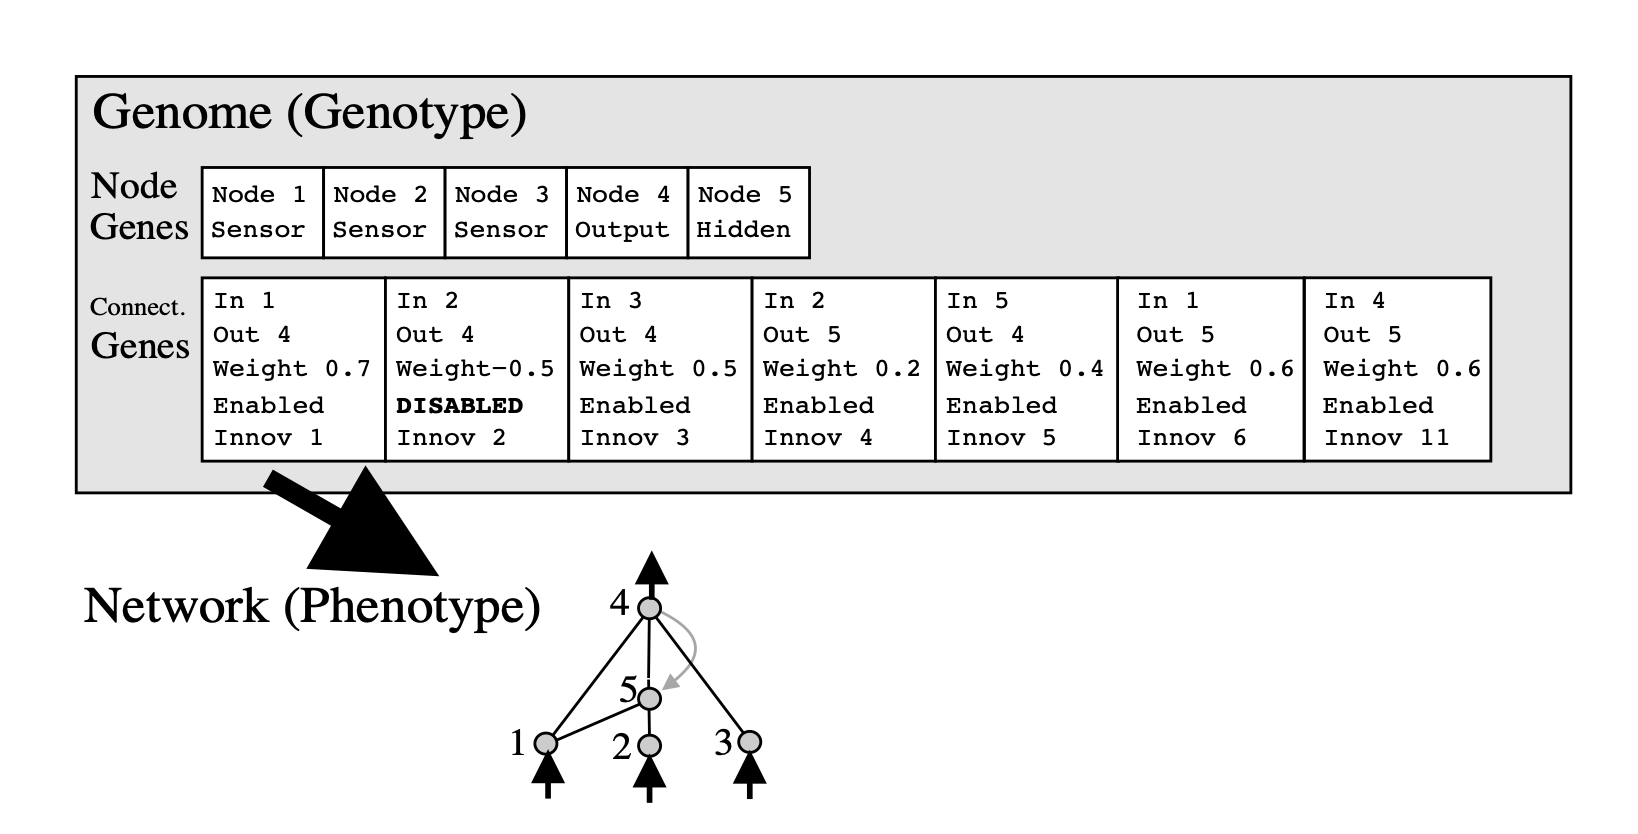
\includegraphics[width=0.85\textwidth]{Figures/genotype_phenotype.png}
\begin{figure}[h]
\centering
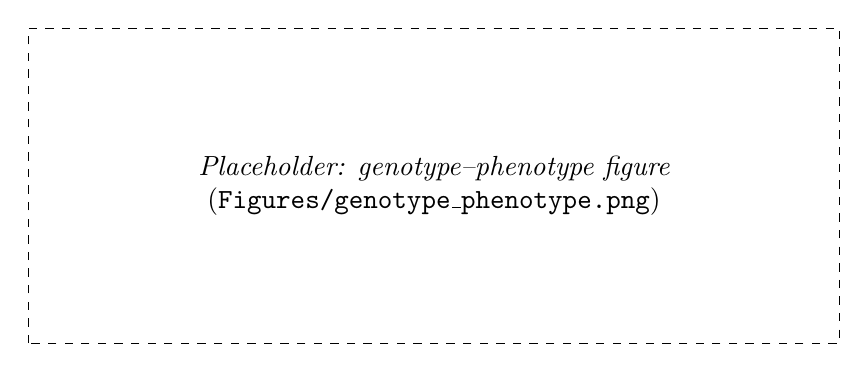
\begin{tikzpicture}
  \draw[dashed] (0,0) rectangle (0.85\textwidth,4cm);
  \node[align=center] at (0.425\textwidth,2cm)
    {\itshape Placeholder: genotype--phenotype figure\\(\texttt{Figures/genotype\_phenotype.png})};
\end{tikzpicture}
\caption{Genotype--phenotype correspondence in NEAT and the structural mutation operator. A node-addition mutation splits an existing connection: the original connection is disabled and two new connections inherit innovation numbers from a global counter.}
\label{fig:genotype-phenotype}
\end{figure}

The second mechanism is speciation.
NEAT partitions the population into species by a compatibility distance that counts excess, disjoint, and weight-difference terms between two genomes.
Genomes compete mainly within their own species, so a fresh structural innovation has time to be tuned before it faces the full population.
The third mechanism is complexification from minimal structure: because the population starts with no hidden nodes, networks grow only through mutation, which biases the search toward parsimonious topologies without a hand-tuned complexity penalty.

% TODO: Here we need to provide more context because we have not introduced the reader to the enviornment that we are solving
% The evolved network is the controller, that is, the policy that maps observations to actions.
% Because NEAT optimises this policy by selection alone, it needs no gradient and no differentiable reward signal; it ranks genomes directly by a scalar fitness accumulated over an episodic roll-out.
% This makes it suitable for continuous-control tasks, where the evaluation is a roll-out of the policy in a physics environment and the fitness is the return accumulated over that roll-out (\cite{stanley_evolving_2002}).


% ---------------------------------------------------------------------
% 1.3
% ---------------------------------------------------------------------
\subsection{Activation Functions}
\label{subsec:activation-functions} 
% PURPOSE: define the activation function as a design choice; show that
%          heterogeneity helps -- the groundwork HA-NEAT exploits.
% COVER:
%   - standard ANNs use one activation function across all nodes
%   - ReLU as canonical example (+ your tikz ReLU figure)
%   - mixed / heterogeneous activations beat homogeneous ones
%   - SANN: gradient-based precedent for per-neuron activation
%   - neuronal diversity outperforms homogeneous nets
% ANCHORS: \cite{nair_rectified_nodate}, \cite{krizhevsky_imagenet_2012},
%          \cite{dubey_activation_2022}, \cite{tutuncuoglu_neuronlevel_2025},
%          \cite{choudhary_neuronal_2023}   <- rescued citation
% REUSE:   your existing "Activation functions" subsection, near-verbatim,
%          including the ReLU tikz figure.
% DECISION: keep the one biological sentence (\cite{song_highly_2005},
%           synapse variation cell-to-cell) as light motivation, or cut it
%           for consistency with dropping the biology thread?
% ENDS:    "...so what if the activation function itself could evolve?"

% >>> write 1.3 here  (reuse ReLU figure)

% short explanation what activation functions are:

An activation function is a nonlinear function applied to each neuron's weighted input. 
This nonlinearity is necessary for depth to add expressive power: the composition of linear maps is itself linear, 
so a network without activation functions computes a single linear map regardless of its number of layers \parencite{dubey_activation_2022}.
The Rectified Linear Unit (ReLU) \parencite{nair_rectified_2010} is the canonical example: it outputs zero for negative inputs and the input itself for positive ones.

Common activation functions that are often used are the identity function, the sigmoid function, the hyperbolic tangent, the Rectified Linear Unit (ReLU), and the sine function.
These functions differ along the properties commonly used to characterise activation functions: output range, monotonicity, and smoothness \parencite{dubey_activation_2022}.
The sigmoid and the hyperbolic tangent are the classical choices, both bounded and saturating. The sigmoid maps to $(0,1)$ and $\tanh$ to the zero-centred interval $(-1,1)$ \parencite{dubey_activation_2022}.
Their saturation at large inputs later motivated the Rectified Linear Unit, which is piecewise-linear, unbounded above, and cheap to evaluate \parencite{nair_rectified_2010}.
ReLU has since become the default activation in deep learning. In deep convolutional networks such as AlexNet it accelerated training over saturating units \parencite{krizhevsky_imagenet_2012,ramachandran_searching_2017}.
The sine function is uncommon in feedforward training but has a longer history in neuroevolution, where periodic activations let a network encode repeating and symmetric structure compactly \parencite{stanley_compositional_2007}.
The identity function applies no nonlinearity. A network which uses only identity functions as activation functions collapses to a linear model \parencite{dubey_activation_2022}.
The choice of activation therefore shapes both which mappings a network can represent and how efficiently it learns them \parencite{dubey_activation_2022}.
Table~\ref{tab:activation-functions} summarises the five functions and their properties. Figure~\ref{fig:activation-functions} plots them.
% Table~\ref{tab:activation-functions} lists the activation functions used in this thesis.
% The five functions differ along the properties commonly used to characterise them: output range, monotonicity, and smoothness (\cite{dubey_activation_2022}).
% The sigmoid and the hyperbolic tangent are the classical choices for neuroevolution, both bounded and saturating; the sigmoid maps to $(0,1)$ and $\tanh$ to the zero-centred interval $(-1,1)$ (\cite{stanley_evolving_2002}).
% Their saturation at large inputs motivated the Rectified Linear Unit, which is piecewise-linear, unbounded above, and cheap to evaluate (\cite{nair_rectified_2010}); in deep convolutional networks such as AlexNet it accelerated training over saturating units (\cite{krizhevsky_imagenet_2012,ramachandran_searching_2017}).
% The sine function is uncommon in feedforward training but has a longer history in neuroevolution, where periodic activations let a network encode repeating and symmetric structure compactly (\cite{stanley_compositional_2007}).
% The identity function applies no nonlinearity; a network built only from identity units suffers the linear collapse described above.
% Figure~\ref{fig:activation-functions} plots all five functions.

\begin{table}[h]
\centering
\caption{Activation functions used in this thesis and their properties.}
\label{tab:activation-functions}
\begin{tabular}{lllll}
\toprule
\textbf{Function} & \textbf{Formula} & \textbf{Range} & \textbf{Monotone} & \textbf{Smooth} \\
\midrule
Identity  & $f(x)=x$                    & $(-\infty,\infty)$ & yes & yes \\
Sigmoid   & $\sigma(x)=\frac{1}{1+e^{-x}}$ & $(0,1)$          & yes & yes \\
Tanh      & $\tanh(x)$                  & $(-1,1)$           & yes & yes \\
ReLU      & $\mathrm{ReLU}(x)=\max(0,x)$ & $[0,\infty)$       & yes & no  \\
Sine      & $\sin(x)$                   & $[-1,1]$           & no  & yes \\
\bottomrule
\end{tabular}
\end{table}

\begin{figure}[h]
\centering
\includegraphics[width=0.85\textwidth]{Figures/activation_functions.png}
\caption{\revFig{F-05}{Comparison of common activation functions}}
\label{fig:activation-functions}
\end{figure}
% new site here 


Artificial neural networks typically use a single activation function across every node \parencite{dubey_activation_2022}.
That uniformity discards the response diversity of Section~\ref{subsec:structural-differences-in-the-brain-and}, which lets a heterogeneous population of biological neurons encode roughly twice as much information as a homogeneous one \parencite{padmanabhan_intrinsic_2010}.
Training a network with multiple activation functions, a heterogeneous network, recovers part of this advantage.
A survey of activation functions reports that a mixture outperforms standard ReLU or sigmoid networks across a range of tasks \parencite{dubey_activation_2022}. \revAcro{A-05}{Self-Activating Neural Networks (SANN)}, which use gradient descent to learn a distinct activation per neuron, can in theory represent functions that a fixed-activation network of the same depth cannot \parencite{tutuncuoglu_neuronlevel_2025}.

The activation function also shapes the inductive bias of a network, the assumptions a model builds into its hypothesis space before seeing data \parencite{papavasileiou_importance_2017}.
\textcite{papavasileiou_importance_2017} showed that the functional form of the activation directly affects the discriminative ability of an evolved network: Gaussian output units in \revAcro{A-06}{Feature Selective NEAT (FS-NEAT)} and \revAcro{A-07}{FD-NEAT} enabled more accurate feature selection and smaller topologies than sigmoid or ReLU units.
\textcite{papavasileiou_optimizing_2022} extended this to HA-FD-NEAT, which evolves heterogeneity, topology, and input selection jointly, and reported that synchronising a neuron's activation with its connectivity lets evolution match the inductive bias to the task.
Functional diversity therefore serves both to compress topology and to optimise input processing.
Standard NEAT holds a single activation function fixed across every node, so the diversity these results exploit is unavailable to it.
Heterogeneous Activation NEAT (HA-NEAT) makes the activation function itself an evolvable, per-neuron trait.


% Different problems need different mathematical transformations. 

%Creating neural networks with a diverse set of activation functions has shown to  Using a set of AF (relu, sigmoid, swish, tanh) instead of only one activation function can improve efficiency and decrease the size of the neural network. (add some examples here)

% ---------------------------------------------------------------------
% 1.4
% ---------------------------------------------------------------------
\subsection{Heterogeneous Neuroevolution (HA-NEAT)}
\label{subsec:haneat}
% PURPOSE: present HA-NEAT, its parsimony result, and its limitation.
% COVER:
%   - genome extension: per-neuron activation gene + mutation operator,
%     protected by speciation
%   - parsimony result: 50-70% smaller networks
%   - functional form changes inductive bias (FS-/FD-NEAT, HA-FD-NEAT)
%   - LIMITATION: all validated on static / classification data
% ANCHORS: \cite{hagg_evolving_2017}, \cite{papavasileiou_importance_2017},
%          \cite{papavasileiou_optimizing_2022}
% REUSE:   your "Heterogeneous Neuroevolution" subsection, nearly intact.
% ENDS:    "...but only on static data -- the continuous-control domain
%           is open."  (the domain gap)

% >>> write 1.4 here

% The HA-NEAT algorithm (\cite{hagg_evolving_2017}) extends the standard NEAT genome by encoding each neuron's activation function as an additional gene, so that topology, weights, and per-node activation all evolve jointly.
% Its central empirical result is structural parsimony: heterogeneous networks match or exceed the accuracy of homogeneous baselines while using 50\%--70\% fewer nodes and connections (\cite{hagg_evolving_2017}).
% A mutation operator reassigns a node's activation function from a fixed library, which \textcite{hagg_evolving_2017} restricted to the step, ReLU, sigmoid, and Gaussian functions.
% They excluded periodic and negative-output functions such as sine, because these require a different output range and would force the network to rescale node outputs dynamically.
% Swapping an activation changes how the node transforms its input, so the mutation is initially disruptive.
% HA-NEAT therefore reuses NEAT's speciation mechanism to shield the mutant until its weights co-adapt to the new nonlinearity.

% Section~\ref{subsec:activation-functions} showed that the activation function also fixes a network's inductive bias.
% HA-NEAT makes that bias evolvable per neuron, so the reported advantage combines topological compression with a task-adapted functional form (\cite{papavasileiou_optimizing_2022}).
% Every HA-NEAT result to date was obtained on static classification and regression benchmarks.
% Whether the same parsimony and inductive-bias advantages transfer to a temporally extended control task remains open. The next two sections set up that question.


The HA-NEAT algorithm \parencite{hagg_evolving_2017} extends the standard NEAT genome by encoding each neuron's activation function as an additional gene, so that topology, weights, and per-node activation evolve jointly.
Its central empirical result is structural parsimony: heterogeneous networks match or exceed the accuracy of homogeneous baselines while using 50\%--70\% fewer nodes and connections \parencite{hagg_evolving_2017}.
A mutation operator reassigns a node's activation function \revTerm{T-04}{from a library of qualitatively different forms}, such as sine, Gaussian, and ReLU.
Swapping an activation changes how the node transforms its input, so the mutation is initially disruptive.
HA-NEAT therefore reuses NEAT's speciation mechanism to shield the mutant until its weights co-adapt to the new nonlinearity.

Section~\ref{subsec:activation-functions} showed that the activation function also fixes a network's inductive bias.
HA-NEAT makes that bias evolvable per neuron, so the reported advantage combines topological compression with a task-adapted functional form \parencite{papavasileiou_optimizing_2022}.
Every HA-NEAT result to date was obtained on static classification and regression benchmarks.
Whether the same parsimony and inductive-bias advantages transfer to a temporally extended control task remains open. The next two sections set up that question.


% ---------------------------------------------------------------------
% 1.5
% ---------------------------------------------------------------------
\subsection{Direct and Indirect Encoding}
\label{subsec:direct-and-indirect-encoding}
% PURPOSE: justify staying with NEAT's direct, parsimonious encoding.
% COVER:
%   - direct (NEAT/HA-NEAT): explicit genome, parsimony, per-neuron
%     activation control, interpretable
%   - indirect (HyperNEAT/CPPN): abstracts connectivity from geometry,
%     scales to millions of connections, but loses per-neuron control and
%     assumes geometric regularity that locomotion does not offer
%   - why direct encoding fits this thesis
% ANCHORS: \cite{stanley_hypercubebased_2009}, \cite{stanley_compositional_2007}
%          (used here as CONTRAST, not as the chosen method)
% REUSE:   the HyperNEAT/CPPN paragraph relocated out of 1.2, reframed.
% ENDS:    "...therefore this work stays with direct encoding."

% >>> write 1.5 here

Neuroevolution methods differ in how the genome maps to a network, and this choice constrains what the algorithm can control.
NEAT and HA-NEAT use a direct encoding: every node, connection, and (in HA-NEAT) activation function appears explicitly in the genome, so genotype and phenotype grow together.
An indirect encoding severs this correspondence.
The main example is HyperNEAT \parencite{stanley_hypercubebased_2009}, which evolves a Compositional Pattern-Producing Network (CPPN) \parencite{stanley_compositional_2007} that generates each connection weight from the geometric coordinates of its endpoints.
A small CPPN can then specify a network of millions of connections, as long as the task supplies geometric regularity for it to exploit.

We keep the direct encoding, for three reasons.
HA-NEAT assigns each neuron its own activation function, and only a genome that lists neurons explicitly can carry that assignment. A CPPN-generated substrate cannot.
This thesis also treats network size as a measured quantity under selective pressure, and direct encoding keeps genome size equal to network size, whereas an indirect encoding decouples them.
HyperNEAT's own advantages, finally, do not reach this setting.
Its compression pays off only for networks far larger than a locomotion controller \parencite{stanley_hypercubebased_2009}, and its geometric prior fits spatially structured inputs such as a visual field, which the low-dimensional proprioceptive state of Hopper and Walker2D does not supply.
Direct encoding thus preserves the exact properties we evaluate, and the open question is the domain in which to evaluate them.

% ---------------------------------------------------------------------
% 1.6
% ---------------------------------------------------------------------
\subsection{Continuous-Control Benchmarks}
\label{subsec:control-benchmarks}
% PURPOSE: introduce the domain and why it is harder than where
%          (HA-)NEAT was validated.
% COVER:
%   - continuous-control locomotion benchmarks
%   - Hopper and Walker2D  (state here: 11 / 17 observations, 3 / 6 actions)
%   - why harder than classification: high-dim continuous actions,
%     temporal credit assignment, policy-dependent non-stationary state
%     distribution, no labels
%   - MuJoCo locomotion lineage
%   - Brax = JAX reimplementation -> massively parallel evaluation
%     (why this matters for population-based neuroevolution); TensorNEAT
% ANCHORS: \cite{freeman_brax_2021}      [TODO-CITE]
%          \cite{todorov_mujoco_2012}    [TODO-CITE]
%          \cite{brockman_openai_2016}   [TODO-CITE]
%          TensorNEAT                     [TODO-CITE]
% REUSE:   nothing from the old Meta-World text.
% ENDS:    "...yet heterogeneous-activation neuroevolution has never been
%           tested in this domain."

% >>> write 1.6 here

Continuous-control locomotion benchmarks evaluate a policy that outputs real-valued torques for a simulated robot body.
The standard benchmark suite \parencite{brockman_openai_2016,duan_benchmarking_2016} is built on the MuJoCo physics engine \parencite{todorov_mujoco_2012}, whose fast and accurate contact dynamics made physically grounded locomotion tasks tractable for reinforcement-learning research.
\revPlain{P-08}{Two of its canonical tasks anchor this thesis.}
Hopper is a one-legged body that must hop forward without falling. Its state is an $11$-dimensional vector of joint positions and velocities, and its action is a $3$-dimensional torque vector, one per actuated joint.
Walker2D is a planar biped that must walk forward while balancing on two legs. It exposes a $17$-dimensional observation and a $6$-dimensional action.
The two bodies share a kinematic lineage, which makes a single shared controller a plausible target for both tasks. Section~\ref{subsec:problem-formulation} sets out the overlap in detail.

These tasks are qualitatively harder than the static classification, regression, and low-dimensional toy control settings in which HA-NEAT has historically been validated \parencite{hagg_evolving_2017}.
Three properties account for the difficulty.
The action space is high-dimensional and continuous, so the controller outputs real-valued torques instead of a discrete label.
Reward arrives only after a sequence of actions, so credit must be assigned across time.
And the distribution of states the policy encounters is itself a function of the policy, which makes the learning target non-stationary and unlabelled.
A controller that performs well must therefore encode temporally coherent behaviour over an episode.

Population-based neuroevolution is expensive in this domain because every genome must be rolled out over full episodes to estimate its fitness.
Brax \parencite{freeman_brax_2021} reduces this cost by reimplementing MuJoCo-style locomotion in JAX, so that thousands of environment instances run in parallel on a single accelerator and evaluation compiles onto the same device as the search.
This shift made population-based evaluation on locomotion tractable at scales that were previously impractical.
The search algorithm must match that scale.
Classical CPU-bound NEAT libraries do not reach the population sizes and generation counts this study requires.
GPU-native implementations such as TensorNEAT \parencite{wang_tensorized_2024} close the gap by tensorising the evolutionary operators onto the same accelerator that runs the simulation.

Despite the maturity of these benchmarks, heterogeneous-activation neuroevolution has, to our knowledge, never been tested in this domain. Its parsimony and inductive-bias advantages remain established only on the static data of Section~\ref{subsec:haneat}.


% Neuroevolution methods differ in how the genome maps to a network, and this choice constrains what the algorithm can control.
% NEAT and HA-NEAT use a direct encoding: every node, connection, and (in HA-NEAT) activation function appears explicitly in the genome, so genotype and phenotype grow together.
% An indirect encoding severs this correspondence.
% The main example is HyperNEAT (\cite{stanley_hypercubebased_2009}), which evolves a Compositional Pattern-Producing Network (CPPN) (\cite{stanley_compositional_2007}) that generates each connection weight from the geometric coordinates of its endpoints.
% A small CPPN can then specify a network of millions of connections, as long as the task supplies geometric regularity for it to exploit.

% We keep the direct encoding, for three reasons.
% HA-NEAT assigns each neuron its own activation function, and only a genome that lists neurons explicitly can carry that assignment; a CPPN-generated substrate cannot.
% This thesis also treats network size as a measured quantity under selective pressure, and direct encoding keeps genome size equal to network size, whereas an indirect encoding decouples them.
% HyperNEAT's own advantages, finally, do not reach this setting.
% Its compression pays off only for networks far larger than a locomotion controller (\cite{stanley_hypercubebased_2009}), and its geometric prior fits spatially structured inputs such as a visual field, which the low-dimensional proprioceptive state of Hopper and Walker2D does not supply.
% Direct encoding thus preserves the exact properties we evaluate, and the open question is the domain in which to evaluate them.

% ---------------------------------------------------------------------
% 1.7
% ---------------------------------------------------------------------
\subsection{Multi-Task Learning with a Single Shared Network}
\label{subsec:multi-task-learning-with-a-single}
% NOTE: title deliberately avoids "Reinforcement Learning" -- your
%       professor flagged that the old title was not about RL methods.
% PURPOSE: introduce multi-task learning as related work; motivate one
%          shared controller for two environments (evolutionary framing,
%          NOT gradient-based MTRL as *your* method).
% COVER:
%   - multi-task RL landscape as contrast (gradient MTRL, engineered
%     expert modules)
%   - the neuroevolutionary alternative
%   - why one shared network is the harder / more interesting target
%   - shared-network rationale: zero-padded 28-in / 9-out union;
%     Walker2D right-leg ~ Hopper leg kinematic overlap
% ANCHORS: \cite{mclean_multitask_2025}     [TODO-CITE]
%          \cite{hendawy_multitask_2024}    [TODO-CITE]
%          \cite{zhang_mixture--world_2026} (gradient-MTRL contrast)
%          \cite{zhou_neuroevolutionary_2024} [TODO-CITE] (closest
%            evolutionary precedent)
%          \cite{leng_understanding_2025}         <- rescued citation
% REUSE:   essentially new; old Meta-World prose does not survive.
% DECISION: preview the zero-padding mechanics here, or keep 1.7
%           conceptual and detail them in Methodology?
%           (recommendation: keep conceptual here.)
% ENDS:    "...and never as a single shared network."

% >>> write 1.7 here

% TODO: remove last sentence here. We do not want to provide the literature gap/research question in this chapter but in research gap and contribution section.
Multi-task learning is a paradigm where a single model is trained on multiple related tasks simultaneously.
By sharing representations and learning processes, the knowledge gained from one task can help improve the performance and \revBrit{E-03}{generalization} of the others \parencite{zhang_survey_2021}.
Recent empirical analysis of \revAcro{A-09}{Large Language Models (LLMs)} reveals that powerful generalist models naturally develop ``task-specific neurons'' that \revBrit{E-04}{specialize} in distinct functional roles \parencite{leng_understanding_2025}.
This thesis asks whether providing a set of activation functions lets evolution assign such \revBrit{E-05}{specialized} \revPlain{P-06}{mathematical ``personalities'' to specific neurons}. We probe the resulting modularity of the control policy only indirectly, through fitness and activation-usage statistics, with no direct measurement of functional specialisation.

To evaluate the efficacy of heterogeneous activation functions in high-dimensional continuous control, this research uses two Brax locomotion environments \parencite{freeman_brax_2021}: Hopper and Walker2D.
A single evolved network must control both bodies at once using one shared set of weights.
The two tasks require diverse motor skills, from single-leg hopping to bipedal balance and forward propulsion.
This setting suits the study because the two environments share a kinematic lineage while differing in observation dimensionality and action space. A single genome must therefore reuse the same circuitry across two interfaces, and specialising in either one leaves it unable to serve the other.
While approaches such as \revAcro{A-08}{Mixture-of-World (MoW) models} address this heterogeneity by explicitly engineering diverse expert modules \parencite{zhang_mixtureofworld_2026}, this thesis asks whether a heterogeneous NEAT network can reach similar functional modularity on its own, by evolving a population of neurons tailored to the two locomotion tasks.


% Multi-task learning trains a single model on several related tasks at once, so that representations learned on one task can transfer to the others (\cite{zhang_survey_2021}).
% Recent work on large language models reports that generalist networks develop ``task-specific neurons'' that specialise in distinct functional roles (\cite{leng_understanding_2025}), which suggests that a single shared network can develop internal modularity on its own.
% This thesis hypothesises that an evolutionary search over per-neuron activation functions can assign such specialised mathematical ``personalities'' to individual neurons, and thereby modularise a shared control policy without engineered expert modules.

% The challenge is concrete.
% The two environments introduced in Section~\ref{subsec:control-benchmarks} --- Hopper and Walker2D --- differ in both observation and output dimensionality.
% A single shared network must ingest Hopper's $11$-dimensional observation and Walker2D's $17$-dimensional observation through the same input layer, and must produce $3$- versus $6$-dimensional torque outputs through the same output layer, using one shared set of weights.
% The smaller observation must be embedded into the larger input space and the unused output channels masked, so the network sees two different input distributions and drives two different actuator sets while its parameters are selected by a single fitness signal.
% One weight set must therefore encode two motor behaviours --- single-leg hopping and bipedal walking --- whose dynamics overlap only partially.

% Engineered approaches address such heterogeneity by composing distinct expert modules, as in Mixture-of-World models (\cite{zhang_mixtureofworld_2026}).
% This thesis instead asks whether a NEAT-based heterogeneous network can discover comparable functional modularity emergently, by evolving a diverse population of neurons tailored to the two locomotion tasks.

% ---------------------------------------------------------------------
% 1.8
% ---------------------------------------------------------------------
\subsection{Research Gap}
\label{subsec:research-gap-and-contribution}
% PURPOSE: synthesize 1.4 x 1.6 (x 1.7) into the gap; state the
%          contribution; hand off to the methodology.
% COVER:
%   - the gap = heterogeneous-activation neuroevolution (static-data only)
%     INTERSECT multi-task continuous-control locomotion (never done this way)
%   - contribution: one shared neuroevolved network, heterogeneous
%     per-neuron activations, Hopper + Walker2D SIMULTANEOUSLY;
%     the JAX / Brax / TensorNEAT pipeline
%   - the "activation personalities" hypothesis (modularizing the policy)
% ANCHORS: synthesis of 1.4 + 1.6 + 1.7; your own hypothesis
% REUSE:   your "This thesis hypothesizes..." paragraph lands cleanly here.
% ENDS:    "...which sets up the methodology that follows."

% >>> write 1.8 here

Two lines of work meet in this thesis.
Heterogeneous-activation neuroevolution (Section~\ref{subsec:haneat}) shows that letting evolution choose a per-neuron activation function yields smaller networks and a task-adapted inductive bias.
Every such result, however, has been established on static, single-task classification data (Section~\ref{subsec:haneat}).
Continuous-control locomotion (Section~\ref{subsec:control-benchmarks}) is a mature benchmark domain for neuroevolution, yet it has only ever been approached with a homogeneous activation function fixed across all nodes.
Whether activation heterogeneity confers an advantage in a temporally extended control setting remains an open question.
The same holds for \emph{emergent modularity}: the spontaneous specialisation of neurons within a single shared network that must solve more than one task at once.
That intersection is the gap this thesis addresses.
Closing it requires three things: an interface that carries two observation and action spaces of different size, \revTerm{T-05}{an activation library whose members differ in shape}, and an evolutionary setup that compares the homogeneous and heterogeneous variants on matched terms.
Section~\ref{sec:methodology} specifies each in turn.


% =====================================================================
%  [ OPEN SLOT ]  Additional topics you mentioned go here. Send the
%  titles + anchor papers and I will insert / renumber them without
%  breaking the red thread.
% =====================================================================

% \section{Literature Review}

% \subsection{Activation functions}
% Artificial neural networks typicall only use one activation functions across every node. In biological neural networks, the synapses between two cells vary from cell to cell (\cite{song_highly_2005}). ANNs, on the other hand, typically use the very same activation function in one single across the  network. 

% An activation function that is often used, because of its simplicity and its properties, is the Rectified Linear Unit (ReLU) (\cite{nair_rectified_nodate}). ReLU outputs 0 for negative inputs and the input itself for positive inputs. Mathematically, it is defined as $\mathrm{ReLU}(x)=\max(0,x)$. ReLu can accelerate the convergence of Stochastic Gradient Descend, as its gradient is always one for positive inputs. This allows the network to learn faster. A simple ANN trained on the CIFAR-10 dataset achieved six times faster a 25\% training error rate than using the tanh function (\cite{krizhevsky_imagenet_2012}). Figure~\ref{fig:relu-plot} shows a schematic plot of this function. 

% \begin{figure}[h]\centering\begin{tikzpicture}[scale=0.9]  \draw[->] (-3,0) -- (3,0) node[right] {$x$};  \draw[->] (0,-0.5) -- (0,3) node[above] {$\mathrm{ReLU}(x)$};  \draw[thick] (-3,0) -- (0,0);  \draw[thick] (0,0) -- (3,3);\end{tikzpicture}\caption{Schematic plot of the Rectified Linear Unit (ReLU) activation function.}\label{fig:relu-plot}\end{figure}

% \newpage

% % Different problems need different mathematical transformations. 
% However, training a neural network with multiple activation functions (heterogeneous network) has shown to improve the performance of ANNs in different scenarious. A comprehensive survey provided evidence that a mix of activation functions performs better than standard ReLu or sigmoid networks (\cite{dubey_activation_2022}). Furthermore, a self developing method called Self-Activating Neural Networks (SANN) that uses gradient descend to evole a unique AF for every Neuron shows that networks can theoretically represent functions that would otherwise require deeper architectures with fixed activation functions (\cite{tutuncuoglu_neuronlevel_2025}).

% %Creating neural networks with a diverse set of activation functions has shown to  Using a set of AF (relu, sigmoid, swish, tanh) instead of only one activation function can improve efficiency and decrease the size of the neural network. (add some examples here)

% \subsection{Neuroevolution of augmenting topoflogies}

% Typical ANNs stick to the initialized topology and then adjust their weights throughout the training process. Thus, we are stuck optimizing weights for a pre-determined structure. In contrast to this static approach, the Neuroevolution of Augmenting Topologies algorithm (NEAT) introduces a dynamic evolutionary based framework that optimizes both synaptic weights and network topology simultaneously (\cite{stanley_evolving_2002}). The NEAT algorithm is based on evolutionary learning theory. It allows for the organic emergence of topological structures and starts out with a population of uniform ANNs with zero hidden nodes. New structures (nodes and connections) are introduced with mutation throughout the learning process. This approach ensures that the algorithm starts searching for solutions in low dimensions first

% To manage the increasing structural diversity between the ANNs, NEAT utilizes historical markings to align gene crossover between differing topologies. Additionally, it employs speciation to protect new topological innovations, allowing new structures to survive and develope before competing against other solutions of the population.

% While NEAT starts out with a small search spaces by starting with minimal topology, scaling to higher dimensions remains a challenge. To overcome this bottleneck, \cite{stanley_hypercubebased_2009} introduced Hypercube-based NeuroEvolution of Augmenting Topologies (HyperNEAT), which utilizes an indirect encoding method based on Compositional Pattern Producing Networks (CPPNs) (\cite{stanley_compositional_2007}). A CPPN operates as a mapping system where geometric coordinates, such as x and y, serve as inputs to determine the output at that specific location. Unlike standard neural networks that typically use a single activation function, CPPNs utilize a diverse set of functions like gaussian, sine, and sigmoid. This variety enables the network to capture geometric regularities like symmetry and repetition. By exploiting the geometric regularities of the task domain HyperNEAT abstracts the connectivity pattern rather than optimizing each connection individually. This allows the algorithm to enable the evolution of functional networks with millions of connections. 

% \subsection{Heterogeneous Neuroevolution}
% The Heterogeneous Activation NEAT algorithm (HA-NEAT) (\cite{hagg_evolving_2017}) advances the standard NEAT algorithm. It proves empirically that heterogeneous ANNs are structuraly more efficient than bigger ones. The integration of diverse activation functions enables more efficient neural networks. A smaller neural network (less nodes and weights) produces similar or even better accuracy than bigger neural networks with homogenous activation functions. In their experiments, hetergoenous networks were often 50\% - 70\% smaller (in terms of topological size) compared to homogenous baselines. To accomplish this, HA-NEAT adds to the traditional NEAT genome by encoding the activation function of each neuron as a specific gene. This allowing the evolutionary process to select from a library of functions (e.g., Sine, Gaussian, ReLU) alongside topology and weights. This approach introduces a new mutation operator that alters a node's activation function, utilizing NEAT's existing speciation mechanism to protect these potentially disruptive but innovative mathematical changes until they optimize.

% In addition to structural parsimony, the choice of activation function is a critical aspect that significantly changes the inductive bias of a network. \cite{papavasileiou_importance_2017} showed that the choice of functional form directly affects the discriminative ability of an algorithm. The use of Gaussian output units in Feature Selective NEAT (FS-NEAT) and FD-NEAT enabled more accurate feature selection and the evolution of smaller topologies than Sigmoid or ReLU units. This implies that the advantage of heterogeneity is not merely a consequence of size reduction but also a means of optimizing input processing.

% In line with this, \cite{papavasileiou_optimizing_2022} proposed HA-FD-NEAT, which evolves the heterogeneity, topology, and input selection of a neural network. The results of their study show that the synchronization of a neuron's properties with its connectivity enables the evolution of a particular task's inductive bias. The identification of optimal architectures is seemingly dependent on this combination, in which functional diversity is a means of both topological compression and accurate feature relevance.




%Compositional Pattern Producing Networks (CPPNs) offer a robust method for abstracting biological development. They encode complex spatial patterns without the need to simulate local interactions or growth over time. A CPPN operates as a mapping system where geometric coordinates, such as x and y, serve as inputs to determine the output at that specific location . Unlike standard neural networks that typically use a single activation function, CPPNs utilize a diverse set of functions like Gaussian, sine, and sigmoid. This variety enables the network to capture geometric regularities like symmetry and repetition. Additionally, because the phenotype is defined by a continuous function, patterns can be represented at infinite resolution

%To bridge the gap between smaller and complex neural networks \cite{stanley_compositional_2007} introduced Compositional Pattern Producing Networks (CPPNs). 

%Hypercube based NEAT (HyperNEAT) introduces a algorithm that uses indirect encoding to approach this problem \cite{stanley_hypercubebased_2009}. It evolves a pattern-producing network that itself generates the weights of the final Network that is used to solve the problem.

% \subsection{Multi-Task Reinforcement Learning}
% This thesis hypothesizes that by providing a diverse library of activation functions, evolution can explicitly assign these specialized mathematical "personalities" to specific neurons, thereby organically modularizing the control policy. 

% To evaluate the efficacy of heterogeneous activation functions in high-dimensional continuous control, this research makes use of the Meta-World benchmark (\cite{yu_meta-world_2021}). Meta-World presents a suite of 50 distinct robotic manipulation tasks (MT50) that share a common physical simulated robot arm. It requires the acquisition of diverse motor skills, ranging from precise pick-and-place operations to dynamic object manipulation. 

% The benchmark is suited for this study because it introduces significant heterogeneity in both observation spaces and task dynamics, challenging the agent to generalize across different environments. While state-of-the-art approaches like Mixture-of-World (MoW) models address this heterogeneity by explicitly engineering diverse expert modules (\cite{zhang_mixture--world_2026}), this thesis posits that an Heterogenous Neural Network based on the NEAT algorithm can emergently discover similar functional modularity by evolving a diverse population of neurons tailored to specific sub-tasks within the Meta-World environment.

% \section{Literature Review}
% \subsection{Neuroplasticity}
% Unlike Artificial Neural Networks (ANNs), the (human) brain is a non-static and continuously changing network. Neural cells form new connections throughout time and rewire to adapt to the current environment (\cite{pascualleone_plastic_2005,holtmaat_experience-dependent_2009}). Cells are constantly rewiring and find new pathways to best represent the environment the human body is experiencing. Human learning yields measurable structural plasticity, demonstrating that adaptation is supported by tangible architectural reconfiguration of the brain (\cite{draganski_changes_2004}). 

% Neuro-plasiticy is the reason why animals and humans are able to learn new behaviours and patterns through experience. It describes the process of neural networks forming. Human brain cells are able to create new connections between each other. (\cite{hebb_organization_1949}, \cite{bliss_lomo_1973})

% In contrast, ANNs typically rely on static connections. We create the structure of the neural, network before we start training it. Hence, the topology of the ANN is fixed. Therefore, it is not possible for artificial intelligence (AI) to create new connections to different neurons while being trained. We solely rely on adapting the weights of the ANN through a process called backpropagation (\cite{rumelhart_learning_1986}). Inspired by biological learning, backpropagation can be seen as a simplified mathematical way to change synaptic strengths: the network keeps its wiring, but the "strength" of each connection is adjusted during training. In the brain, synaptic change is also not random but gated by local activity and chemical signals, which provides a useful inspiration even if the biological mechanism is not identical to backpropagation (\cite{fremaux_neuromodulated_2016,roelfsema_three-factor_2018}). 

% Gradient descend tries to find an optimal solution where a loss function is minimized. This training regime works well when data is available in large batches and the task distribution is mostly stationary. However, the underlying data often changes its distribution throughout time (data shift), which is common in real-world environments and can lead to ANNs whose learned statistical assumptions become outdated (\cite{quinonero-candela_dataset_2009,gama_survey_2014}).


% \subsection{Catastrophic Forgetting}
% Another difference between ANNs and classical neura networks becomes visible once tasks arrive sequentially. Homogeneous ANNs tend to overwrite previously learned representations (Catastrophic forgetting), whereas biological systems maintain a much richer toolbox of mechanisms to protect and reorganize knowledge over time. Catastrophic forgetting (also called catastrophic interference) describes the tendency of gradient-based ANNs to lose performance on previously learned tasks when trained sequentially on new tasks. Early analyses suggest that this is not a minor side-effect but a structural property of distributed representations: when multiple tasks share parameters, learning task $B$ will typically move weights into a region that is no longer optimal for task $A$ (\cite{mccloskey_catastrophic_1989,french_catastrophic_1999}). In practice, this makes "learning from a stream" fundamentally different from the standard independent identically distributed (i.i.d.) setting that most deep learning pipelines assume.

% In machine learning, this gap motivates continual learning methods that explicitly reduce forgetting (\cite{kirkpatrick_overcoming_2017,parisi_continual_2019}) and approaches that re-introduce fast, local plasticity into networks, i.e., making parts of the connectivity itself adapt online (\cite{miconi_differentiable_2018}). \cite{lillo_activation_2026} found that the AF choice is an "architecture-agnostic lever for mitigating plasticity loss" in continual learning setting. Furthermore, mathematical and neuronal diversity, much like that observed in biological systems, significantly outperforms homogeneous architectures by enhancing the expressiveness and adaptability of artificial neural networks. (\cite{choudhary_neuronal_2023}). 

% While catastrophic forgetting is often introduced on supervised benchmarks, it becomes particularly relevant in reinforcement learning. The data distribution is non-stationary because it depends on the current policy, and even small updates can change the visited state distribution. This makes stability-plasticity trade-offs harder and increases the pressure on replay, regularization, and modular architectures (\cite{khetarpal_continual_2020,schwarz_progress_2018}).

% %From a continual learning perspective, modern approaches can be roughly grouped into (i) rehearsal/replay, (ii) regularization-based stabilization, and (iii) architectural strategies. Replay methods keep a small memory buffer (or a generative model) and interleave old experiences with new ones, which is conceptually close to what is done in many RL agents via experience replay (\cite{rolnick_experience_2019}). Regularization-based methods, such as Elastic Weight Consolidation (EWC), constrain updates along directions that are estimated to be important for past tasks (\cite{kirkpatrick_overcoming_2017}), while related methods like Synaptic Intelligence track parameter importance online (\cite{zenke_continual_2017}). Architectural strategies reduce interference by allocating new capacity over time, for example via progressive networks that grow task-specific modules while preserving earlier ones (\cite{rusu_progressive_2016}). Knowledge-distillation based methods, such as Learning without Forgetting, fit naturally into this picture by retaining old function outputs while adapting to a new dataset (\cite{li_learning_2017}).



% \subsection{Activation functions}
% Artificial neural networks typicall only use one activation functions across every node. In biological neural networks, the synapses between two cells vary from cell to cell (\cite{song_highly_2005}). ANNs, on the other hand, typically use the very same activation function in one single across the  network. 

% An activation function that is often used, because of its simplicity and its properties, is the Rectified Linear Unit (ReLU) (\cite{nair_rectified_nodate}). ReLU outputs 0 for negative inputs and the input itself for positive inputs. Mathematically, it is defined as $\mathrm{ReLU}(x)=\max(0,x)$. ReLu can accelerate the convergence of Stochastic Gradient Descend, as its gradient is always one for positive inputs. This allows the network to learn faster. A simple ANN trained on the CIFAR-10 dataset achieved six times faster a 25\% training error rate than using the tanh function (\cite{krizhevsky_imagenet_2012}). Figure~\ref{fig:relu-plot} shows a schematic plot of this function. 

% \begin{figure}[h]\centering\begin{tikzpicture}[scale=0.9]  \draw[->] (-3,0) -- (3,0) node[right] {$x$};  \draw[->] (0,-0.5) -- (0,3) node[above] {$\mathrm{ReLU}(x)$};  \draw[thick] (-3,0) -- (0,0);  \draw[thick] (0,0) -- (3,3);\end{tikzpicture}\caption{Schematic plot of the Rectified Linear Unit (ReLU) activation function.}\label{fig:relu-plot}\end{figure}

% \newpage

% % Different problems need different mathematical transformations. 
% However, training a neural network with multiple activation functions (heterogeneous network) has shown to improve the performance of ANNs in different scenarious. A comprehensive survey provided evidence that a mix of activation functions performs better than standard ReLu or sigmoid networks (\cite{dubey_activation_2022}). Furthermore, a self developing method called Self-Activating Neural Networks (SANN) that uses gradient descend to evole a unique AF for every Neuron shows that networks can theoretically represent functions that would otherwise require deeper architectures with fixed activation functions (\cite{tutuncuoglu_neuronlevel_2025}).

% %Creating neural networks with a diverse set of activation functions has shown to  Using a set of AF (relu, sigmoid, swish, tanh) instead of only one activation function can improve efficiency and decrease the size of the neural network. (add some examples here)

% Another key difference becomes visible once tasks arrive sequentially: standard ANNs tend to overwrite previously learned representations (catastrophic forgetting), whereas biological systems maintain a much richer toolbox of mechanisms to protect and reorganize knowledge over time. In machine learning, this gap motivates continual learning methods that explicitly reduce forgetting (\cite{kirkpatrick_overcoming_2017,parisi_continual_2019}) and approaches that re-introduce fast, local plasticity into networks, i.e., making parts of the connectivity itself adapt online (\cite{miconi_differentiable_2018}). \cite{lillo_activation_2026} found that the AF choice is an "architecture-agnostic lever for mitigating plasticity loss" in continual learning setting. Furthermore, neuronal diversity like in biological systems has shown evidence to outperform homogenous ones (\cite{choudhary_neuronal_2023})

% \subsection{Neuroevolution of augmenting topologies}

% Typical ANNs stick to the initialized topology and then adjust their weights throughout the training process. Thus, we are stuck optimizing weights for a pre-determined structure. In contrast to this static approach, the Neuroevolution of Augmenting Topologies algorithm (NEAT) introduces a dynamic evolutionary based framework that optimizes both synaptic weights and network topology simultaneously (\cite{stanley_evolving_2002}). The NEAT algorithm is based on evolutionary learning theory. It allows for the organic emergence of topological structures and starts out with a population of uniform ANNs with zero hidden nodes. New structures (nodes and connections) are introduced with mutation throughout the learning process. This approach ensures that the algorithm starts searching for solutions in low dimensions first

% To manage the increasing structural diversity between the ANNs, NEAT utilizes historical markings to align gene crossover between differing topologies. Additionally, it employs speciation to protect new topological innovations, allowing new structures to survive and develope before competing against other solutions of the population.

% While NEAT starts out with a small search spaces by starting with minimal topology, scaling to higher dimensions remains a challenge. To overcome this bottleneck, \cite{stanley_hypercubebased_2009} introduced Hypercube-based NeuroEvolution of Augmenting Topologies (HyperNEAT), which utilizes an indirect encoding method based on Compositional Pattern Producing Networks (CPPNs) (\cite{stanley_compositional_2007}). A CPPN operates as a mapping system where geometric coordinates, such as x and y, serve as inputs to determine the output at that specific location. Unlike standard neural networks that typically use a single activation function, CPPNs utilize a diverse set of functions like gaussian, sine, and sigmoid. This variety enables the network to capture geometric regularities like symmetry and repetition. By exploiting the geometric regularities of the task domain HyperNEAT abstracts the connectivity pattern rather than optimizing each connection individually. This allows the algorithm to enable the evolution of functional networks with millions of connections. 

% \subsection{Heterogeneous Neuroevolution}
% The Heterogeneous Activation NEAT algorithm (HA-NEAT) (\cite{hagg_evolving_2017}) advances the standard NEAT algorithm. It proves empirically that heterogeneous ANNs are structuraly more efficient than bigger ones. The integration of diverse activation functions enables more efficient neural networks. A smaller neural network (less nodes and weights) produces similar or even better accuracy than bigger neural networks with homogenous activation functions. In their experiments, hetergoenous networks were often 50\% - 70\% smaller (in terms of topological size) compared to homogenous baselines. To accomplish this, HA-NEAT adds to the traditional NEAT genome by encoding the activation function of each neuron as a specific gene. This allowing the evolutionary process to select from a library of functions (e.g., Sine, Gaussian, ReLU) alongside topology and weights. This approach introduces a new mutation operator that alters a node's activation function, utilizing NEAT's existing speciation mechanism to protect these potentially disruptive but innovative mathematical changes until they optimize.

% In addition to structural parsimony, the choice of activation function is a critical aspect that significantly changes the inductive bias of a network. \cite{papavasileiou_importance_2017} showed that the choice of functional form directly affects the discriminative ability of an algorithm. The use of Gaussian output units in Feature Selective NEAT (FS-NEAT) and FD-NEAT enabled more accurate feature selection and the evolution of smaller topologies than Sigmoid or ReLU units. This implies that the advantage of heterogeneity is not merely a consequence of size reduction but also a means of optimizing input processing.

% In line with this, \cite{papavasileiou_optimizing_2022} proposed HA-FD-NEAT, which evolves the heterogeneity, topology, and input selection of a neural network. The results of their study show that the synchronization of a neuron's properties with its connectivity enables the evolution of a particular task's inductive bias. The identification of optimal architectures is seemingly dependent on this combination, in which functional diversity is a means of both topological compression and accurate feature relevance.




% %Compositional Pattern Producing Networks (CPPNs) offer a robust method for abstracting biological development. They encode complex spatial patterns without the need to simulate local interactions or growth over time. A CPPN operates as a mapping system where geometric coordinates, such as x and y, serve as inputs to determine the output at that specific location . Unlike standard neural networks that typically use a single activation function, CPPNs utilize a diverse set of functions like Gaussian, sine, and sigmoid. This variety enables the network to capture geometric regularities like symmetry and repetition. Additionally, because the phenotype is defined by a continuous function, patterns can be represented at infinite resolution

% %To bridge the gap between smaller and complex neural networks \cite{stanley_compositional_2007} introduced Compositional Pattern Producing Networks (CPPNs). 

% %Hypercube based NEAT (HyperNEAT) introduces a algorithm that uses indirect encoding to approach this problem \cite{stanley_hypercubebased_2009}. It evolves a pattern-producing network that itself generates the weights of the final Network that is used to solve the problem.

% \subsection{Multi-Task Reinforcement Learning}
% The transition from homogeneous to heterogeneous architectures is necessitated by the "stability-plasticity dilemma," where standard neural networks suffer from catastrophic forgetting as learning new tasks interferes with the weights required for previous ones (\cite{abbasi_sparsity_2022}). Recent empirical analysis of Large Language Models (LLMs) supports this view, revealing that powerful generalist models naturally develop "task-specific neurons" that specialize in distinct functional roles (\cite{leng_understanding_2025}). 

% This thesis hypothesizes that by providing a diverse library of activation functions, evolution can explicitly assign these specialized mathematical "personalities" to specific neurons, thereby organically modularizing the control policy. 

% To evaluate the efficacy of heterogeneous activation functions in high-dimensional continuous control, this research makes use of the Meta-World benchmark (\cite{yu_meta-world_2021}). Meta-World presents a suite of 50 distinct robotic manipulation tasks (MT50) that share a common physical simulated robot arm. It requires the acquisition of diverse motor skills, ranging from precise pick-and-place operations to dynamic object manipulation. 

% The benchmark is suited for this study because it introduces significant heterogeneity in both observation spaces and task dynamics, challenging the agent to generalize across different environments. While state-of-the-art approaches like Mixture-of-World (MoW) models address this heterogeneity by explicitly engineering diverse expert modules (\cite{zhang_mixture--world_2026}), this thesis posits that an Heterogenous Neural Network based on the NEAT algorithm can emergently discover similar functional modularity by evolving a diverse population of neurons tailored to specific sub-tasks within the Meta-World environment.



%Contemporary deep learning predominantly relies on gradient-based optimization methods, such as backpropagation, applied to fixed, pre-defined network topologies. While this paradigm has achieved remarkable success in supervised learning, it inherently assumes that the initialized architecture possesses the optimal inductive bias for the given task.

%In contrast to this static approach, the Neuroevolution of Augmenting Topologies  algorithm introduces a dynamic evolutionary based framework that optimizes both synaptic weights and network topology simultaneously (\cite{stanley_evolving_2002}). Unlike gradient-based methods, NEAT begins with minimal complexity and incrementally adds nodes and connections. 

%While gradient methods typically offer superior sample efficiency in high-dimensional parameter spaces, NEAT provides a distinct advantage in reinforcement learning environments characterized by sparse rewards or deceptive local optima. Crucially, by uncoupling the agent from rigid architectural constraints, NEAT allows for the organic emergence of topological structures, providing a fertile ground for investigaZting how specialized functional modules might evolve without explicit human design.

%While canonical NEAT excels at optimizing topology, it typically relies on a homogeneous set of activation functions—usually sigmoids—thereby assuming a uniform non-linearity suffices for all processing tasks. Addressing this limitation, \cite{hagg_evolving_2017} proposed Heterogeneous Activation NEAT (HA-NEAT), an extension that co-evolves the activation function of individual neurons alongside the network structure and weights. By expanding the genome to include a direct encoding of diverse activation types—such as Gaussian, ReLU, Step, and Sigmoid—HA-NEAT allows the evolutionary process to select the most appropriate local inductive bias for specific network regions. This heterogeneity encourages greater parsimony, producing significantly smaller networks that are less prone to overfitting than their homogeneous counterparts. Crucially for multi-task domains, this diversity facilitates emergent modularity; for example, distinct activation profiles allow the network to organically separate correlated signals into distinct functional pathways, a phenomenon observed where specific sub-networks specialize in partial aspects of the target output.


\section{Methodology}
\label{sec:methodology}

\subsection{Problem Formulation}
\label{subsec:problem-formulation}

This work addresses the multi-task learning problem of evolving a single neuroevolutionary network capable of controlling two continuous-locomotion agents simultaneously: Hopper and Walker2D from the Brax physics suite.
The objective is a single shared neural network that receives observations from either environment, generates the appropriate joint-torque actions, and accumulates reward across both tasks, in place of two separately trained controllers.
A genome's fitness is therefore defined by its combined performance on both environments, evaluated every generation.

The two environments were introduced in Section~\ref{subsec:control-benchmarks}. The dimensions that drive the shared-network design are the observation and action spaces of each environment.
Hopper exposes an 11-dimensional observation and a 3-dimensional action, while Walker2D exposes a 17-dimensional observation and a 6-dimensional action.
Because these dimensions differ, a single fixed-topology network cannot ingest both environments directly, \revGram{G-08}{and it motivates a padding scheme of the neural network}.
The two bodies also overlap anatomically.
Hopper is a single planar leg: a torso with thigh, lower-leg, and foot segments connected by three actuated hinge joints.
Each of Walker2D's two legs follows the same segment and joint layout, with identical joint axes and ranges. Only foot length and actuator strength differ.
Control circuitry evolved for one of these legs can, in principle, drive the other, so the task pair is a suitable setting for a single shared network.

% We pair the two tasks to test for cross-task transfer. Representations acquired on Hopper's simpler locomotion problem might bootstrap performance on Walker2D, and vice versa.
Our hypothesis concerns activation heterogeneity: whether allowing each hidden node to carry its own activation function improves multi-task performance relative to a homogeneous network. We address this question through a controlled comparison of standard NEAT against HA-NEAT in the multi-task setting.


\subsection{Genome Representation and the Padding Scheme}
\label{subsec:genome-representation-and-the-padding-scheme}

Because Hopper and Walker2D differ in observation and action dimensionality, a mechanism is required to present both environments to a single fixed-topology network.
The approach adopted in this work is a union padding scheme: the network is constructed with 17 input nodes and 6 output nodes, corresponding to the maximum observation and action dimensions across both tasks.
This design was chosen over modular sub-networks to keep the shared-structure argument clean. Any shared structure discovered by evolution arises from optimisation pressure alone, not from an architecture decision.

Formally, given a network $f: \mathbb{R}^{17} \rightarrow \mathbb{R}^{6}$, the task-specific action functions are defined as:

\[a_{\text{Hopper}} = f([\mathbf{o}_{\text{Hopper}}; \mathbf{0}_{6}])_{1:3}\]
\[\revNota{N-05}{a_{\text{Walker}} = f(\mathbf{o}_{\text{Walker}})_{1:6}}\]

where $[\cdot; \cdot]$ denotes concatenation and the subscript denotes output slicing.
For Hopper, the 11-dimensional observation vector is zero-padded to 17 dimensions before being presented to the network, and only the first 3 of the 6 output dimensions are used as actions.
For Walker2D, all inputs and outputs are used directly without modification.

\begin{figure}[h]
    \centering
    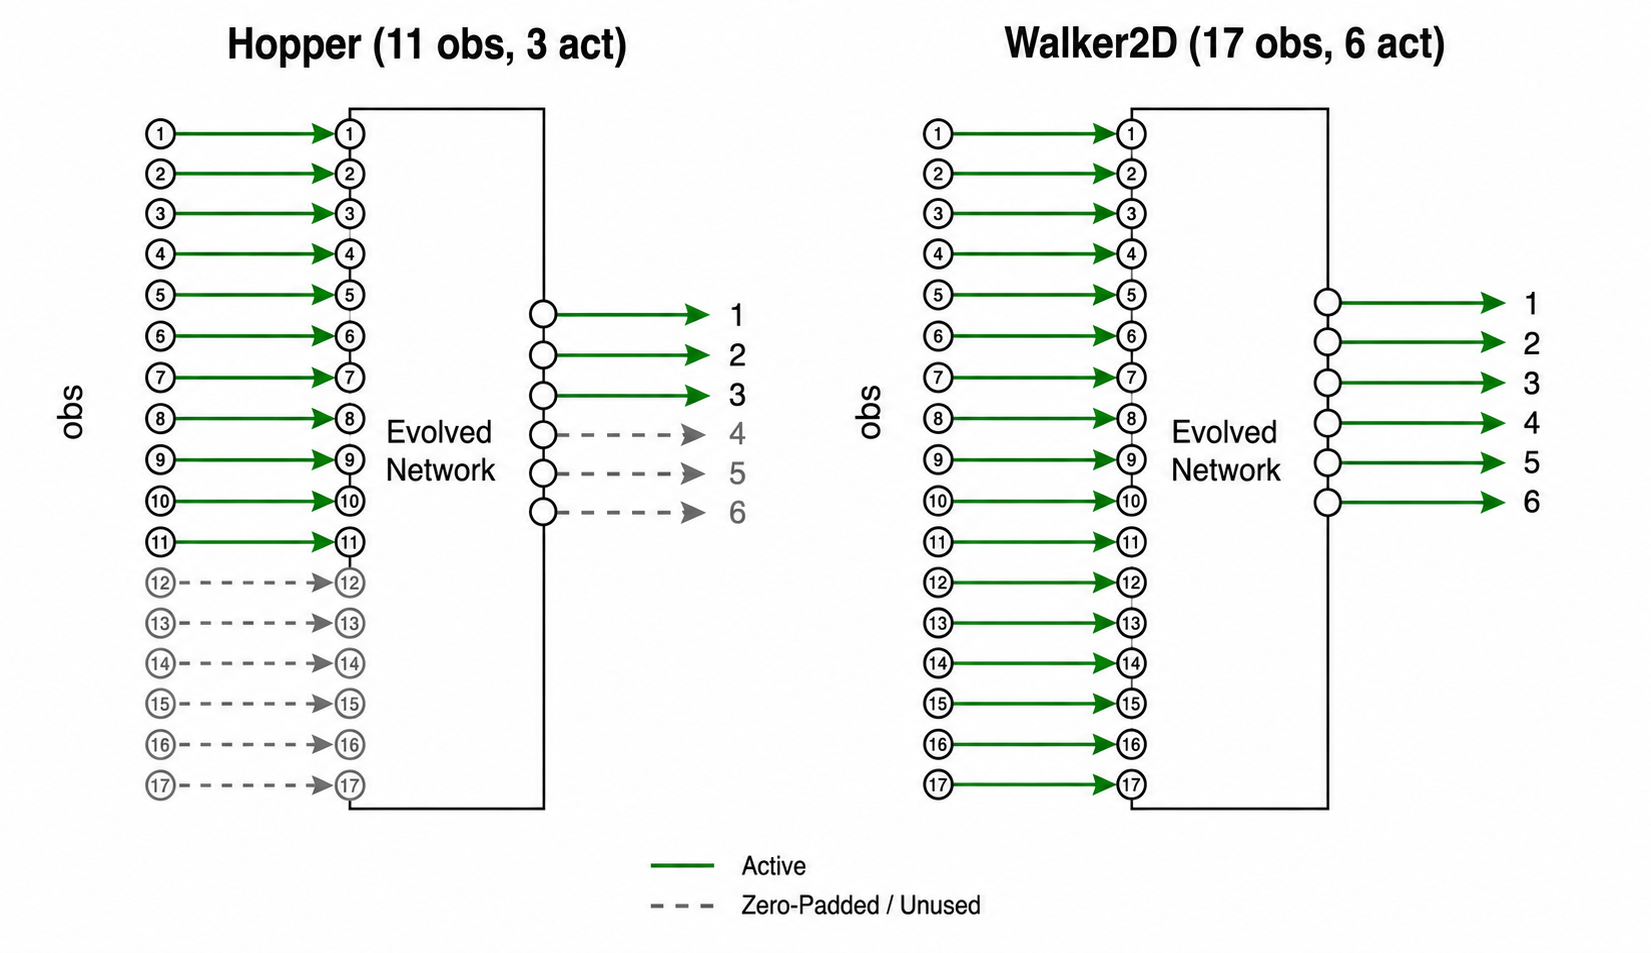
\includegraphics[width=0.85\textwidth]{Figures/Network_newv2.png}
    \caption{The shared network interface for the multi-task setup. The same evolved network serves both tasks. For Hopper, inputs 12--17 receive zero padding and outputs 4--6 are unused. Walker2D uses all 17 inputs and all 6 outputs natively.}
    \label{fig:network-architecture}
\end{figure}

The zero-padded input positions are constant during Hopper episodes, so Hopper applies no selection pressure on the connections leaving them.
The network may learn to route Hopper-relevant computation through the first 11 input nodes while reserving the remaining 6 for Walker2D-specific processing, or it may discover shared representations spanning both input regions.
Figure~\ref{fig:network-architecture} illustrates this shared interface.

At the implementation level, nodes are stored as a $[N_{\max} \times 4]$ array encoding index, bias, aggregation function, and activation function per node.
Connections are stored as a $[C_{\max} \times 4]$ array encoding source index, destination index, historical marker, and weight per connection.
Inactive positions carry NaN in the first column of either array. A gene is active exactly when its first entry is not NaN.


\subsection{Algorithm Design: HA-NEAT}
\label{subsec:algorithm-design-ha-neat}

Section~\ref{subsec:haneat} motivated heterogeneous activations and the speciation protection that shields them. This section specifies the algorithm that implements both.

\subsubsection{NEAT Foundation}
\label{subsubsec:neat-foundation}

NEAT evolves network topology and weights jointly through historical marking, speciation, and complexification from minimal structure, as introduced in Section~\ref{subsec:neuroevolution-of-augmenting-topologies-neat}.
We restate here only the details the HA-NEAT extensions build on.

Each genome encodes a variable-topology neural network as two gene lists: node genes and connection genes.
A node gene stores a unique index, a bias value, an aggregation function, and an activation function.
A connection gene stores source and destination node indices, a historical marker, and a weight value.
The array-level storage of these gene lists is described in Section~\ref{subsec:genome-representation-and-the-padding-scheme}.

The population is partitioned into species based on genetic distance.
Two connection genes are \emph{homologous} when they carry the same historical marker, meaning both descend from the same ancestral structural mutation. A gene whose marker appears in only one genome is non-homologous.
For each pair of genomes, the distance function aligns connection genes by their identifying attributes, counts non-homologous genes, and computes attribute differences on homologous genes.
Where the encoding carries a historical marker, the identifying attributes are that marker together with the (source, destination) index pair. Otherwise they are the index pair alone. Section~\ref{subsec:experimental-conditions} contrasts the two identity schemes.
The distance between two genomes is

\[d = \frac{D \cdot c_d + \sum_{i \in H} \delta_i \cdot c_w}{\max(n_1, n_2)}\]

where $D$ denotes the count of non-homologous genes, \revNota{N-02}{$H$ denotes the set of homologous gene pairs}, \revNota{N-03}{$\delta_i$ is the attribute distance for pair $i$}, \revNota{N-01}{$c_d$ and $c_w$ weight the two terms} (values in Table~\ref{tab:hyperparameters}), and $n_1$, $n_2$ are the gene counts of each genome.
\revClarity{L-02}{The distance is computed separately over node genes, aligned by node index, and over connection genes, aligned by their identifying attributes, and the two values are summed.}
For a homologous connection pair, $\delta_i$ is the absolute weight difference $|w_1 - w_2|$.
For a homologous node pair it is $|b_1 - b_2| + \mathbb{1}[\text{agg}_1 \neq \text{agg}_2] + \mathbb{1}[\text{act}_1 \neq \text{act}_2]$, the absolute bias difference plus one unit for each mismatched aggregation or activation function.
An activation mutation therefore raises the genetic distance twice over: directly, through this activation term, and indirectly, through the marker reassignment of Section~\ref{subsubsec:ha-neat-extensions}.
This form follows the TensorNEAT \parencite{wang_tensorized_2024} implementation and merges the separate disjoint and excess terms of the original NEAT formulation into the single count $D$.
It also divides both terms by $\max(n_1, n_2)$, whereas the original formulation averages attribute differences over homologous pairs only. \revClarity{L-05}{Attribute differences therefore contribute less to the distance in large genomes than under the original definition.}
Genomes whose total distance falls below the compatibility threshold $\theta$ (Table~\ref{tab:hyperparameters}) are assigned to the same species.

Within each species, the top fraction of genomes, set by the survival threshold (Table~\ref{tab:hyperparameters}), produces offspring through crossover and mutation.
During crossover, genes are aligned by historical marker. Homologous genes are inherited randomly from either parent, and non-homologous genes come from the fitter parent.

% NEAT (NeuroEvolution of Augmenting Topologies)~\cite{stanley2002evolving} evolves both the topology and the weights of neural networks through three mechanisms: 
% historical marking of genes for alignment during crossover, speciation to protect structural innovation, and complexification from minimal initial topologies. 
% We summarise it here only to the extent needed to contextualise the HA-NEAT extensions.

% Each genome encodes a variable-topology neural network as two gene lists: node genes and connection genes. A node gene stores a unique index, a bias value, an aggregation function, and an activation function. A connection gene stores source and destination node indices, a historical marker, and a weight value. In the TensorNEAT implementation used in this work~\cite{TODO:tensorneat}, active genes occupy the first rows of fixed-size arrays, and inactive positions are filled with NaN. This padding convention enables batched operations across a population of genomes with different topologies under JAX's static-shape compilation model~\cite{TODO:jax}.

% The population is partitioned into species by genetic distance. For each pair of genomes, the distance function aligns connection genes by historical marker, counts non-homologous (disjoint and excess) genes, and computes attribute differences on homologous genes. The distance between two genomes is
% \begin{equation}
%     d = \frac{D \cdot c_d + \sum_{i \in H} \delta_i \cdot c_w}{\max(n_1, n_2)},
% \end{equation}
% where $D$ is the count of non-homologous genes, $H$ is the set of homologous gene pairs, $\delta_i$ is the attribute distance for pair $i$, $c_d = 1.0$ and $c_w = 0.4$ weight disjoint and weight differences respectively, and $n_1$, $n_2$ are the gene counts of each genome. Genomes whose distance falls below the compatibility threshold $\theta = 1.0$ are assigned to the same species.

% Within each species, the top fraction of genomes, set by the survival threshold, produces offspring through crossover and mutation. During crossover, the fitter parent contributes the structural backbone: homologous genes are inherited randomly from either parent, and all non-homologous genes (disjoint and excess) are inherited from the fitter parent.

\subsubsection{HA-NEAT Extensions}
\label{subsubsec:ha-neat-extensions}

HA-NEAT extends the standard NEAT algorithm with three modifications, all encapsulated within the mutation operator.
The speciation-driven evolutionary loop, crossover, and distance computation remain unchanged.
Each modification is described in turn.

\begin{enumerate}
    \item \textbf{Random activation assignment upon node creation.} In standard NEAT, a newly added node receives the default activation function ($\tanh$). HA-NEAT instead assigns a random activation function drawn uniformly from $\mathcal{A} = \{\tanh, \sigma, \text{ReLU}, \sin, \text{identity}\}$ at node creation. This introduces immediate functional diversity: the new node contributes a non-trivial transformation from its first generation, avoiding the evolutionary delay of waiting for a separate activation mutation.
    
    \item \textbf{Controlled activation mutation with speciation protection.} With probability $p_{\text{act}}$ (Table~\ref{tab:hyperparameters}) per genome per generation, exactly one randomly selected hidden node has its activation function replaced by a function selected from
    $\mathcal{A}$ with equal probability \revTerm{T-06}{across all elements of the palette}. Upon this mutation, all connections attached to the mutated node receive new historical markers from a pre-allocated pool, increasing the genetic distance between the mutated genome and its relatives. This causes the speciation mechanism to place the mutant into a separate species, protecting it from competitive elimination before its weights can co-adapt to the new activation landscape. Section~\ref{subsec:implementation-stack} details the pre-allocated marker pool and the compilation constraint that motivates it.
    
    \item \textbf{Suppression of standard activation mutation.} Standard NEAT applies per-node activation mutation with independent probability during value mutation. HA-NEAT disables this mechanism: the activation column is saved before value mutation and restored afterward, ensuring that only the controlled one-node-per-generation mechanism modifies activations. Unprotected activation changes, i.e. those without corresponding marker reassignment, would lack the speciation shield, exposing functionally disrupted genomes to immediate competitive pressure.
\end{enumerate}


\subsection{Fitness Evaluation}
\label{subsec:fitness-evaluation}

A critical design decision in multi-task neuroevolution is how to aggregate performance across tasks into a single selection signal.
Each generation, every genome in the population is evaluated on both Hopper and Walker2D through the following pipeline:

\begin{enumerate}
    \item \textbf{Decode.} The genome's node and connection arrays are transformed into an executable network representation via topological sort and adjacency matrix construction.
    \item \textbf{Evaluate per task.} The network controls each environment for 1,000 timesteps. Each task uses an independent random key derived deterministically from the genome's evaluation key, ensuring reproducible episode generation across runs.
    \item \textbf{\revBrit{E-06}{Normalize.}} Each raw per-task return is divided by a fixed task-specific constant that accounts for the differing reward scales across environments: 3000 for Hopper and 5000 for Walker2D. We chose these constants ourselves. No published benchmark supplies them. Each sits at the order of magnitude of a strong single-task return in its environment, so a normalised score of 1.0 corresponds to strong single-task competence.
    \item \textbf{Aggregate via the normalised minimum.} The two normalised per-task scores are collapsed into a scalar by taking their minimum.
\end{enumerate}

Formally, writing $r_{\text{Hopper}}$ and $r_{\text{Walker2D}}$ for the raw per-task returns, the fitness of a genome is

\[\text{fit} = \min\!\left(\frac{r_{\text{Hopper}}}{3000},\ \frac{r_{\text{Walker2D}}}{5000}\right).\]

The choice of the minimum follows one principle: an aggregation must not reward \revBrit{E-07}{single-task specialization}.
Walker2D's reward scale substantially exceeds Hopper's, and a sum of the normalised scores allows a genome to attain a high aggregate value by excelling at one task while neglecting the other.
A product drives the aggregate toward zero only if one score collapses entirely. Short of that it still permits substantial imbalance, because a strong score on one task multiplicatively compensates for a weak but nonzero score on the other.
The minimum ties a genome's fitness to its \emph{worse} task, so a network earns reward only once it is competent on both environments at once.
Our argument for the minimum is therefore structural: of the three aggregators, it alone cannot reward a genome for neglecting a task.
We defer the empirical support to the aggregation calibration experiment (Section~\ref{subsec:calibration}), which confirms both weaknesses. Sum and product aggregation there produced genomes that scored well on the aggregate while neglecting one task, an outcome the minimum excludes by construction.

\subsection{Network Architecture}
\label{subsec:network-architecture}

All networks are initialised with a minimal topology: 17 input nodes connected directly to 6 output nodes, with no hidden nodes.
This follows the NEAT principle of complexification: structural complexity emerges through mutation and selection pressure rather than through designer assumptions about required network depth or width.

Output nodes apply a $\tanh$ activation to bound their values within $[-1, 1]$.
This constraint is necessary because Brax environments interpret actions as normalised joint torques: each action dimension specifies the magnitude and direction of force applied to a joint actuator, bounded to the unit interval.

Hidden nodes use per-node activation functions.
In the standard NEAT condition, all hidden nodes use $\tanh$.
In the HA-NEAT condition, \revTerm{T-07}{the activation palette} $\mathcal{A} = \{\tanh, \sigma, \text{ReLU}, \sin, \text{identity}\}$ enables heterogeneous internal representations.
The individual activation functions were selected for their complementary computational properties:

\begin{itemize}
    \item \textbf{Tanh and sigmoid ($\sigma$)}: Bounded and smooth, these functions are suitable for gating behaviour and saturation dynamics, where network outputs must be constrained within a fixed range.
    \item \textbf{ReLU}: One-sided and non-saturating, unbounded in the positive domain \parencite{nair_rectified_2010}. In the small evolved topologies of this study it supplies rectified, piecewise-linear control signals. The depth-related benefits reported for deep architectures do not apply at this scale.
    \item \textbf{Sin}: Periodic by nature, sinusoidal activation is capable of encoding oscillatory patterns, a property of particular relevance to rhythmic locomotion, where joint trajectories follow approximately periodic profiles.
    \item \textbf{Identity}: A linear pass-through that enables skip connections and linear sub-networks, allowing the evolved topology to incorporate proportional control pathways without nonlinear distortion.
\end{itemize}

% The hypothesis underlying the heterogeneous palette is that a network benefits from composing these nonlinearities (periodic functions for gait timing, saturating functions for balance, and linear functions for proportional control), whereas a homogeneous $\tanh$ network must approximate all such behaviours through a single nonlinearity, potentially requiring greater structural complexity.

All hidden nodes employ sum aggregation.
That is, \revNota{N-04}{the pre-activation value of a node is computed as the sum of incoming weighted signals plus a bias term}.
Formally, for node $j$ with incoming connections from the set of source nodes $\mathcal{I}_j$:

\[z_j = \phi_j\left(b_j + \sum_{i \in \mathcal{I}_j} w_{ij} \cdot v_i\right)\]

where $\phi_j \in \mathcal{A}$ denotes the node's activation function, $b_j$ is the bias, $w_{ij}$ are connection weights, and $v_i$ are the output values of source nodes.

\subsection{Implementation Stack}
\label{subsec:implementation-stack}

The experiments are built upon TensorNEAT \parencite{wang_tensorized_2024}, a GPU-accelerated NEAT implementation constructed on JAX.
TensorNEAT encodes the entire evolutionary pipeline (population initialisation, mutation, crossover, speciation, fitness evaluation, and selection) as JAX-transformable functions, compiling to a single XLA computation graph via \texttt{jax.jit} executed entirely on the GPU without CPU-GPU data transfers during the evolutionary loop.
Population-level operations are vectorised using \texttt{jax.vmap}, eliminating Python-level loops over the population.
This end-to-end GPU execution was the primary motivation for selecting TensorNEAT over classical CPU-based NEAT implementations such as NEAT-Python.

JAX's static-shape requirement also constrains the HA-NEAT mutation operator (Section~\ref{subsubsec:ha-neat-extensions}).
The mutation operator pre-allocates $3 + C_{\max}$ historical markers per genome per generation, where $C_{\max}$ denotes the maximum number of connections: the first three serve the standard structural mutations, and the remaining $C_{\max}$ cover the worst case of an activation mutation that re-marks every connection incident to a single node.
Pre-allocation keeps marker assignment free of dynamic memory allocation inside the compiled graph.

Brax \parencite{freeman_brax_2021} provides the physics backend, implementing rigid-body simulation as differentiable JAX functions that integrate directly with TensorNEAT's JIT-compiled evaluation loop.
% Brax exposes several dynamics pipelines.
% Early runs used the \texttt{generalized} backend, but it permitted a physics exploit in Walker2D: genomes learned to drive limbs through the floor and accumulate spurious forward reward without producing genuine locomotion.
% All reported experiments therefore use the MJX backend (MuJoCo-XLA), which enforces proper contact dynamics and removes this exploit.
The combination of JAX-native evolution and JAX-native simulation eliminates the host-device transfer bottleneck that limits frameworks in which the evolutionary algorithm runs on the CPU while fitness evaluation runs on the GPU.

Experiment tracking is implemented using MLflow.
Each run logs per-generation metrics including maximum, mean, minimum, and standard deviation of fitness across the population, alongside valid genome count, generation wall-clock time, species count, stagnation counter, and the node and connection counts of the best genome.
Per-task fitness scores for the best genome are tracked separately for Hopper and Walker2D, enabling post-hoc analysis of task-specific performance trajectories and the degree to which the shared network specialises toward one environment over the other.
The aggregated \texttt{best\_fitness} metric records the normalised minimum defined in Section~\ref{subsec:fitness-evaluation}, so its per-generation trajectory tracks the worse of the two normalised per-task rewards.

% \begin{table}[h]
% \centering
% \caption{MLflow Metrics Logged Per Generation}
% \label{tab:mlflow_metrics}
% \begin{tabular}{lll}
% \toprule
% \textbf{Metric} & \textbf{Description} & \textbf{Scope} \\
% \midrule
% \texttt{fitness/max}          & Maximum fitness in population          & Population \\
% \texttt{fitness/mean}         & Mean fitness in population             & Population \\
% \texttt{fitness/min}          & Minimum fitness in population          & Population \\
% \texttt{fitness/std}          & Standard deviation of fitness          & Population \\
% \texttt{fitness/valid\_count} & Number of successfully evaluated genomes & Population \\
% \texttt{fitness/hopper}       & Best genome reward on Hopper           & Best genome \\
% \texttt{fitness/walker2d}     & Best genome reward on Walker2D         & Best genome \\
% \texttt{best\_fitness}        & Aggregated fitness of best genome (normalised minimum) & Best genome \\
% \texttt{neat/n\_species}      & Number of active species               & Population \\
% \texttt{stability/stagnation\_counter} & Generations without improvement & Population \\
% \texttt{neat/best\_genome\_n\_nodes}  & Node count of best genome       & Best genome \\
% \texttt{neat/best\_genome\_n\_conns}  & Connection count of best genome & Best genome \\
% \texttt{neat/avg\_genome\_n\_conns}   & Mean connection count across population & Population \\
% \texttt{cost\_time\_ms}       & Wall-clock time per generation (ms)    & Run \\
% \bottomrule
% \end{tabular}
% \end{table}

\section{Experimental Settings}
\label{sec:experimental-settings}

\subsection{Environment Details}
\label{subsec:environment-details}

Table~\ref{tab:env-specs} presents the specifications of both evaluation environments.

\begin{table}[h]
\centering
\caption{\revFig{F-06a}{Environment Specifications}}
\label{tab:env-specs}
\begin{tabular}{lll}
\toprule
\textbf{Property} & \textbf{Hopper} & \textbf{Walker2D} \\
\midrule
Observation dimensions & 11 & 17 \\
Action dimensions & 3 & 6 \\
Padded input dimensions & 17 (6 zeros appended) & 17 (native) \\
Padded output dimensions & 6 (last 3 unused) & 6 (native) \\
Episode length & 1,000 timesteps & 1,000 timesteps \\
Action range & [-1, 1] (continuous) & [-1, 1] (continuous) \\
\revAcro{A-01}{Simulator} & Brax v0.14.1 (MJX) & Brax v0.14.1 (MJX) \\
\bottomrule
\end{tabular}
\end{table}

Both environments reward forward locomotion while penalising energy expenditure and falls.
Hopper terminates an episode early if the torso height falls below a threshold or the torso tilts beyond a critical angle. Walker2D applies analogous termination conditions for its bipedal stance.
The reward structures differ in scale: Walker2D typically yields higher cumulative rewards than Hopper for equivalent locomotion quality.
This scale asymmetry motivates the per-task normalisation constants (3000 for Hopper, 5000 for Walker2D) and the normalised-minimum aggregation defined in Section~\ref{subsec:fitness-evaluation}.

\subsection{Experimental Conditions}
\label{subsec:experimental-conditions}

The experiment compares three conditions, all operating within the multi-task Hopper + Walker2D setting:

\begin{enumerate}
    \item \textbf{Multi-Task NEAT (baseline).} Standard NEAT with homogeneous $\tanh$ activation functions on all hidden nodes. This condition uses \texttt{DefaultConn}, which carries no historical markers. Gene identity is instead given by the (source, destination) index pair, so crossover and distance align connection genes by structure rather than by marker. Absent marker reassignment the two identity schemes agree almost everywhere, since a connection's endpoints never change after creation. They diverge in one case only: when two lineages independently create the same connection, the marker scheme counts two distinct genes and the index-pair scheme counts one. The standard per-node activation mutation mechanism is active but has no practical effect, since only one activation option is available.

    \item \textbf{Multi-Task HA-NEAT (treatment).} HA-NEAT with heterogeneous activations \revTerm{T-08}{drawn from the palette} $\mathcal{A}$. This condition uses \texttt{OriginConn} with historical markers. Activation mutation occurs at most once per genome per generation, with speciation protection via marker reassignment as described in Section~\ref{subsubsec:ha-neat-extensions}.

    \item \textbf{HA-NEAT ablation (tanh only).} The full HA-NEAT algorithm (\texttt{OriginConn}, controlled activation mutation, and marker reassignment) restricted to a single activation function, $\tanh$. Activation mutation still fires with probability $p_{\text{act}}$ per genome per generation. With a single option available the activation change itself has no functional effect, but the accompanying marker reassignment still occurs. This condition isolates HA-NEAT's structural machinery from its activation diversity: it tests whether an advantage of the treatment requires heterogeneity itself, \revClarity{L-04}{or whether the surrounding speciation machinery already produces it}.
\end{enumerate}

All three conditions use identical population sizes, generation limits, structural mutation rates, and evaluation procedures (Table~\ref{tab:hyperparameters}).
The independent variable is the activation function regime: homogeneous activations, heterogeneous activations with speciation protection, and the ablation that retains the speciation machinery without heterogeneity.
The dependent variables are:

\begin{itemize}
    \item \textbf{Per-task performance}: Each champion's normalised return on Hopper and Walker2D individually, taken as a seed-level mean over the 20 re-evaluation episodes per task, and used to identify which task binds the normalised minimum, that is, which environment limits a genome's aggregate fitness.
    \item \textbf{Genome complexity}: \revTerm{T-13}{The number of active nodes and connections in the best genome}, the structural cost of the evolved solution.
    \item \textbf{Species dynamics}: The number of active species, a proxy for population diversity.
    \item \textbf{Activation composition} (HA-NEAT only): The distribution of activation functions among the hidden nodes of the final champions, measuring whether the evolved networks exercise the heterogeneity the treatment provides.
\end{itemize}

\subsection{Hyperparameters}
\label{subsec:hyperparameters}

Table~\ref{tab:hyperparameters} lists the evolutionary hyperparameters used across the three experimental conditions.
The values are taken from the run parameters logged in MLflow and are identical across all 90 runs of the main study.

\begin{table}[h]
\centering
\caption{\revFig{F-06b}{Evolutionary Hyperparameters}}
\label{tab:hyperparameters}
\begin{tabular}{ll}
\toprule
\textbf{Parameter} & \textbf{Value} \\
\midrule
Population size & 200 \\
Generation limit & 750 \\
\revFig{F-07}{Fitness target} & 10{,}000 \\
Max nodes per genome & 50 \\
Max connections per genome & 200 \\
Maximum species count & 10 \\
Compatibility threshold ($\theta$) & 0.3 \\
Distance coefficients ($c_d$ / $c_w$) & 1.0 / 0.4 \\
Survival threshold & 0.3 \\
Max species stagnation & 40 \\
Species elitism & 2 \\
Genome elitism & 2 \\
Connection add probability & 0.2 \\
Connection delete probability & 0.2 \\
Node add probability & 0.1 \\
Node delete probability & 0.1 \\
Bias init mean / std & 0.0 / 1.0 \\
Bias mutate power / rate & 0.15 / 0.2 \\
Bias replace rate & 0.015 \\
Weight init mean / std & 0.0 / 1.0 \\
Weight mutate power / rate & 0.15 / 0.2 \\
Weight replace rate & 0.015 \\
\midrule
\textbf{HA-NEAT specific} & \\
Activation mutation rate ($p_{\text{act}}$) & 0.1 \\
\revTerm{T-09}{Activation palette} & $\{\tanh, \sigma, \text{ReLU}, \sin, \text{identity}\}$ \\
Standard activation replace rate & 0.0 (disabled) \\
Historical marker reassignment & Enabled (via OriginConn) \\
\bottomrule
\end{tabular}
\end{table}

The compatibility threshold was set empirically.
Earlier large-population experiments compared thresholds of 0.3 and 0.5, and $\theta = 0.3$ was carried over to the main study.
At population 200 this setting filled the configured maximum of 10 species in every condition (Section~\ref{sec:main-complexity}), so the species count sat at its cap and never tracked the threshold. Carrying $\theta$ across the population-size difference therefore remains an assumption of the design.
The survival threshold dictates that the top 30\% of each species produces offspring, creating within-species selection pressure while speciation protects structural diversity across the population as a whole.
The fitness target of 10{,}000 lies far outside the attainable range of the normalised-minimum objective, so no run stopped early. Every run completed the full 750 generations.\footnote{One NEAT run (seed 5213) was aborted at generation 324 and re-run to completion. The truncated run is excluded from all analyses.}

\subsection{Preliminary Calibration Experiments}
\label{subsec:calibration}

Two preliminary experiments calibrated the design of the main study before its full seed grid was run.
The first, the aggregation calibration experiment, compared the three candidate ways of collapsing the two normalised per-task scores into a scalar: their sum, their product, and their minimum.
The grid covered two algorithms, three population sizes, and two generation budgets at a single seed, yielding twelve best genomes per aggregation.
Sum and product permit a genome to score well on the aggregate while neglecting one task. The most extreme case reached a normalised Hopper score of 1.04 while its Walker2D score collapsed to 0.17 (Figure~\ref{fig:aggregation-calibration}).
Consistent with this structural weakness, the minimum produced the smallest mean gap between a genome's stronger and weaker task (0.11, against 0.20 for sum and 0.18 for product) and the highest average weaker-task score.
Because the grid used a single seed we read these differences as a tendency. The decisive argument is structural.
\revBrit{E-08}{The minimum cannot reward specialization}, and it was therefore adopted as the selection signal defined in Section~\ref{subsec:fitness-evaluation}.
The second, the training-budget calibration runs, evolved larger populations \revFig{F-04}{(1024 to 4096 genomes) for up to 2000 generations} and tracked how far best fitness continued to improve.
These runs reached on average 91--93\% of their eventual 2000-generation best by generation 750, and the improvement rate per 100 generations fell four- to five-fold after generation 700 (Figure~\ref{fig:budget-calibration}).
A 750-generation budget therefore captures the large majority of attainable fitness within the diminishing-returns regime, while making the 30-seed, three-condition design of the main study computationally tractable.
The main-study runs at population 200 decelerate even earlier than the calibration runs, so the budget transfers across the population-size difference.

\begin{figure}[h]
    \centering
    \includegraphics[width=0.95\textwidth]{Figures/aggregation_calibration.png}
    \caption{Aggregation calibration experiment (twelve best genomes per aggregation, single-seed grid). (a) Mean normalised score of each genome's stronger and weaker task under sum, minimum, and product aggregation. The minimum yields the smallest stronger--weaker gap and the highest weaker-task score. (b) Per-task profile of each best genome. The dashed diagonal marks balanced performance. Sum and product permit strongly lopsided genomes, including one sum-aggregation genome with a normalised Hopper score of 1.04 and a Walker2D score of 0.17.}
    \label{fig:aggregation-calibration}
\end{figure}

\begin{figure}[h]
    \centering
    \includegraphics[width=0.95\textwidth]{Figures/budget_calibration.png}
    \caption{Training-budget calibration. (a) Best-so-far normalised-minimum fitness against generation for the calibration runs (population 4096, up to 2000 generations). The dashed vertical line marks generation 750. (b) The same curves for the main study (population 200, 750 generations). Improvement rates fall four- to five-fold after generation 700 in every condition, and the smaller main-study populations decelerate earlier than the calibration runs, supporting the 750-generation budget.}
    \label{fig:budget-calibration}
\end{figure}

\subsection{Evaluation Protocol}
\label{subsec:evaluation-protocol}

Each experimental condition was repeated across 30 independent runs. All three conditions used the same 30 random seeds.
The seed list, the full run configuration, and the analysis code are available at \url{https://github.com/SvenGoerdes/tensorneat}.
At $\alpha = 0.05$ and 80\% power, this sample size can detect effects of roughly Cohen's $d \geq 0.74$ with non-parametric tests, while remaining computationally tractable given the cost of population-based neuroevolution on GPU hardware.

Performance is measured at three levels:

\begin{enumerate}
    \item \textbf{Per-generation tracking.} The training pipeline logs the dependent variables of Section~\ref{subsec:experimental-conditions} every generation, alongside population-level fitness statistics (maximum, mean, minimum, and standard deviation). The exception is activation composition, which we compute once from the saved champion genomes.
    \item \textbf{Final performance.} The best genome of each run was re-evaluated after training over 20 episodes per task with fresh random seeds, and the run's score is the normalised minimum of the two per-task re-evaluation means. Training fitness rests on a single episode and is therefore a noisy estimate of policy quality. The re-evaluation removes this noise from the between-condition comparison. Scores are reported as median and interquartile range across the 30 independent runs, and these seed-level values (one per run) are the unit of all statistical analysis.
    \item \textbf{Learning dynamics.} Fitness-over-generation curves, averaged across runs with 95\% confidence bands, to characterise convergence speed and stability.
\end{enumerate}

Statistical comparison across the three conditions uses a Kruskal--Wallis omnibus test ($\alpha = 0.05$) on the seed-level re-evaluation scores, followed by Holm-corrected pairwise Mann--Whitney tests.
Non-parametric tests are appropriate because evolutionary run outcomes are not guaranteed to follow a normal distribution and do not reliably support parametric assumptions.
Each pairwise contrast is accompanied by a Hodges--Lehmann shift estimate with a bootstrap 95\% confidence interval and by Cliff's $\delta$ as an effect size, and equivalence testing (two one-sided tests) complements the significance tests where the question is whether conditions perform the same.

\subsection{Compute Resources}
\label{subsec:compute-resources}

All experiments were conducted on a single compute node with the specifications listed in Table~\ref{tab:compute-node}.

\begin{table}[h]
\centering
\caption{\revFig{F-06c}{Compute Node Specifications}}
\label{tab:compute-node}
\begin{tabular}{ll}
\toprule
\textbf{Component} & \textbf{Specification} \\
\midrule
CPU & AMD Threadripper 7970X (32 cores, 64 threads) \\
RAM & 251 GB \\
GPU & 2$\times$ NVIDIA RTX A6000 (48 GB VRAM each) \\
CUDA & 12.4 \\
Software & JAX 0.9.1, Brax 0.14.1, Python 3.11 \\
\bottomrule
\end{tabular}
\end{table}

Each evolutionary run utilises a single GPU.
The dual-GPU configuration enables two independent runs to execute in parallel, halving the wall-clock time required for the full experimental campaign.
Across the 90 main-study runs, a single run took a median of roughly 3.4~h (mean 3.8~h), for a campaign total of about 340 GPU-hours.
JIT compilation of the evolutionary step occurs once at the start of each run. Subsequent generations execute the compiled XLA graph without recompilation overhead, with the exception of topology-triggered recompilation events that occur when the population's maximum genome size changes.

%\section{Background}

% \section{Methodology}

% \subsection{Problem Formulation}


% The pairing of Hopper and Walker2D is deliberate: both are planar locomotion domains with related lower-limb mechanics, but different body complexity and control demands. Hopper can be interpreted as a constrained single-leg locomotor, whereas Walker2D requires coordinated bilateral stepping. This creates a useful transfer setting: structural regularities (e.g., balance, forward propulsion, leg extension/flexion timing) can be shared, while increased task complexity still demands specialization. The central hypothesis is that HA-NEAT can discover shared substructures and task-specific neuronal roles without manually engineered modularization.

% \subsection{Algorithm Design (HA-NEAT)}
% The method builds on canonical NEAT by evolving not only topology and connection weights, but also neuron-level activation functions (heterogeneous activation NEAT, HA-NEAT). Each genome contains:
% \begin{itemize}
%     \item node genes (node id, type, activation-function id),
%     \item connection genes (in-node, out-node, weight, enabled flag, innovation id).
% \end{itemize}

% Compared to vanilla NEAT, the key extension is an \textit{activation mutation} operator that can change a hidden node's activation function from a predefined library (e.g., ReLU, Tanh, Sigmoid, Gaussian, Sine, Identity). This allows local nonlinearities to co-evolve with topology.

% To support cross-environment evaluation with one genotype, all networks use a unified I/O interface. Inputs are padded to 28 dimensions and outputs to 9 dimensions. For each environment, only task-valid features and actuators are populated; all non-applicable entries are set to zero (zero-masking). Concretely, a Hopper observation/action pair is embedded into the 28/9 vector with deterministic index mapping, and Walker2D uses the same global index system. During rollout, invalid action channels are masked out before being passed to the simulator. This preserves one genome space while allowing task-specific sparsity.

% Mutation and crossover follow NEAT principles with innovation tracking for homologous alignment. Structural mutations include add-node and add-connection; parametric mutations perturb weights; activation mutations alter local transfer functions. Crossover combines matching genes by innovation number and inherits disjoint/excess genes under the configured fitness-parent rule. Speciation uses compatibility distance over structural and parametric differences to protect innovation and prevent immediate elimination of novel topologies.

% \subsection{Fitness Evaluation}
% Each candidate genome is evaluated in both environments within the same generation. Let $R_{\text{H}}$ and $R_{\text{W}}$ denote episode returns (or mean returns over repeated evaluation episodes) for Hopper and Walker2D. To make scales comparable, rewards are normalised by environment-specific solved thresholds $\tau_{\text{H}}$ and $\tau_{\text{W}}$:
% \[
% \hat{R}_{\text{H}}=\frac{R_{\text{H}}}{\tau_{\text{H}}},\qquad
% \hat{R}_{\text{W}}=\frac{R_{\text{W}}}{\tau_{\text{W}}}.
% \]
% The primary scalar fitness is then
% \[
% F=\frac{\hat{R}_{\text{H}}+\hat{R}_{\text{W}}}{2},
% \]
% which equally weights both tasks and discourages specialization to only one environment.

% This aggregation yields a standard single-objective evolutionary loop while still reflecting balanced multi-task competence. As an extension, the same pipeline can be converted into a Pareto formulation with objectives $(\hat{R}_{\text{H}},\hat{R}_{\text{W}})$ and optimized using NSGA-II to explicitly trace trade-offs between task-specific and joint performance.

% \subsection{Network Architecture}
% The phenotype network is represented through a padded graph view that is compatible with a fixed-size adjacency-matrix implementation. At initialization, $\texttt{init\_hidden\_layers=()}$ creates a minimal topology: direct input-to-output connectivity in NEAT style, no hidden layer prior, and random initial weights. This biases search toward simple policies first.

% Complexification then grows topology over generations by selectively inserting new hidden nodes and edges. Insertion of a node splits an existing edge, preserving functional continuity while increasing representational capacity. Add-connection mutations create shortcuts or recurrently useful pathways (if recurrence is enabled by configuration). Because hidden nodes also carry activation-function genes, structural growth and nonlinear diversification are coupled: new subnetworks can emerge with distinct inductive biases for different control motifs (e.g., near-linear stabilization vs.
% nonlinear gait timing).

% Under the padded 28-input/9-output interface, the adjacency representation remains constant in shape across tasks, while the active computational subgraph differs via masking. This allows one evolving topology to host both shared pathways and sparse, task-specific branches.

% \subsection{Implementation Stack}
% The implementation uses TensorNEAT on top of JAX, with Brax as the physics backend. This stack is selected for efficient batched neuroevolution in continuous control. JAX enables vectorized population evaluation and just-in-time (JIT) compilation of rollout and fitness code paths. Brax provides differentiable, accelerator-friendly rigid-body simulation and integrates naturally with JAX tensors.

% The practical advantage is reduced host-device overhead: policy execution, simulation stepping, and fitness aggregation can run in a compiled on-device pipeline rather than frequent CPU--GPU synchronization. For evolutionary methods that evaluate many genomes per generation, this substantially improves throughput and makes repeated multi-run experiments tractable.

% \section{Experimental settings}

% \subsection{Environment Details}
% Table~\ref{tab:env-details} summarizes the two tasks used in this thesis. Both are episodic continuous-control locomotion benchmarks with forward-progress rewards and instability-based terminations.

% \begin{table}[h]
% \centering
% \caption{Environment configuration used for multi-task training and evaluation.}
% \label{tab:env-details}
% \begin{tabular}{lcc}
% \hline
% Property & Hopper & Walker2D \\
% \hline
% Observation dimension & 11 & 17 \\
% Action dimension & 3 & 6 \\
% Padded input dimension & 28 & 28 \\
% Padded output dimension & 9 & 9 \\
% Primary reward signal & Forward locomotion & Forward locomotion \\
% Episode length (max steps) & 1000 & 1000 \\
% Termination & Fall/instability or timeout & Fall/instability or timeout \\
% \hline
% \end{tabular}
% \end{table}

% \subsection{Hyperparameters}
% All evolutionary hyperparameters are fixed across conditions unless explicitly stated otherwise. Table~\ref{tab:hyperparams} lists the core settings.

% \begin{table}[h]
% \centering
% \caption{Core HA-NEAT hyperparameters.}
% \label{tab:hyperparams}
% \begin{tabular}{ll}
% \hline
% Hyperparameter & Value \\
% \hline
% Population size & 512 \\
% Number of generations & 300 \\
% Compatibility threshold $\delta_t$ & 3.0 \\
% Species target & 15 \\
% Crossover rate & 0.75 \\
% Weight mutation rate & 0.80 \\
% Add-node mutation rate & 0.03 \\
% Add-connection mutation rate & 0.05 \\
% Activation mutation rate & 0.10 \\
% Elitism (per species) & 1 \\
% Stagnation limit & 20 generations \\
% \hline
% \end{tabular}
% \end{table}

% \subsection{Experimental Conditions / Independent Variables}
% The primary independent variable is activation-function heterogeneity. We compare:
% \begin{itemize}
%     \item \textbf{Homogeneous baseline}: all hidden nodes use one fixed activation function (ReLU),
%     \item \textbf{Heterogeneous HA-NEAT}: hidden nodes evolve activation type from a shared library.
% \end{itemize}

% The activation-function library for heterogeneous conditions consists of ReLU, Tanh, Sigmoid, Gaussian, Sine, and Identity. This set mixes saturating and non-saturating nonlinearities, localized and periodic responses, and a linear passthrough option. A secondary condition compares \textit{single-task} evolution (Hopper-only or Walker2D-only fitness) against \textit{multi-task} evolution (joint normalised fitness), to isolate transfer effects.

% \subsection{Evaluation Protocol}
% Each condition is executed with multiple random seeds to quantify stochastic variability. The target protocol is 10 independent runs per condition (minimum acceptable: 5). For each run, we log best-genome fitness per generation, population mean fitness, species count, and topology size statistics (nodes/connections).

% Performance is reported on normalised task return and joint fitness. A run is marked as solved for a task when its best genome reaches or exceeds the corresponding solved threshold. Between-condition comparisons use non-parametric tests (Mann--Whitney U for pairwise comparisons) with effect size reporting (Cliff's $\delta$), and Holm correction when multiple pairwise tests are performed.

% \subsection{Compute Resources}
% All experiments are executed on NOVA DAH 01 equipped with an NVIDIA RTX A6000 GPU (48 GB VRAM). The software stack uses CUDA 12.x with JAX-compatible acceleration. Reporting hardware and CUDA runtime is necessary because population-level JIT execution and simulator throughput are sensitive to device class and driver/runtime compatibility.
\newpage

\section{Results and Discussion}
\label{sec:results-and-discussion}

\subsection{Experimental overview}
\label{subsec:experimental-overview}
We evaluated NEAT and HA-NEAT on a single multi-task control problem: one evolved network must control both the Hopper body (11 observations, 3 actions) and the Walker2D body (17 observations, 6 actions) using the same weights, through the zero-padding and output-slicing interface of Section~\ref{subsec:genome-representation-and-the-padding-scheme}.
The main study compared three conditions: standard NEAT (tanh only), HA-NEAT (per-node activations drawn from tanh, sigmoid, relu, sin, identity), and an ablation running HA-NEAT's full machinery restricted to tanh.
Each condition was evolved at population 200 for 750 generations across 30 independent random seeds, giving 90 runs in total on the MJX (MuJoCo on GPU) physics backend.

The selection signal was the normalised minimum of the two per-task scores\revNota{N-06}{}, $\mathrm{fit} = \min(r_{\text{hopper}}/3000,\, r_{\text{walker2d}}/5000)$, so a genome cannot raise its score by \revBrit{E-11}{specializing} in one body and neglecting the other.
Section~\ref{subsec:fitness-evaluation} gives the rationale for this objective. The calibration study (Section~\ref{subsec:calibration}) justified it empirically against the sum and product alternatives and fixed the 750-generation budget.
Preliminary NEAT-versus-HA-NEAT comparisons shaped the rest of the design. We ran them at populations of 1{,}024--4{,}096 with only two to three seeds per condition. They compared the compatibility thresholds carried into Section~\ref{subsec:hyperparameters}, and their failure to separate the two algorithms at that seed count motivated the 30-seed design and the tanh-only ablation that isolates the mutation machinery from activation diversity. The main study reported here supersedes them.

Every champion was re-evaluated after training over 20 episodes per task, and the resulting seed-level values were the unit of all statistical analysis (Section~\ref{subsec:evaluation-protocol}).

Section~\ref{sec:main-study} reports the head-to-head multi-task fitness across the three conditions, which is the study's primary result.
Section~\ref{sec:main-complexity} examines genome complexity and generational dynamics, Section~\ref{sec:main-tradeoff} the per-task trade-off and multi-task pressure, and Section~\ref{sec:main-activation} activation-function usage within HA-NEAT.
Section~\ref{sec:main-discussion} discusses these analyses together.

\subsection{Multi-task fitness across conditions}
\label{sec:main-study}
For each of the 90 runs we took the best genome, re-evaluated it over 20 episodes per task, and computed its normalised-minimum fitness from the two per-task re-evaluation means, giving $n = 30$ seed-level values per condition.
This re-evaluation is the reference performance metric for the study.

The three conditions performed near-identically (Table~\ref{tab:main-fitness}).
NEAT reached a median fitness of 0.184 \revAcro{A-04}{(IQR $[0.124, 0.253]$)}, HA-NEAT 0.208 ($[0.152, 0.276]$), and the ablation 0.199 ($[0.152, 0.258]$).
A Kruskal--Wallis test found no difference across the three conditions ($H = 1.48$, $p = 0.476$, $\revNota{N-07}{\varepsilon^2 \approx 0}$).
Pairwise, every contrast was small and every interval straddled zero: NEAT versus HA-NEAT (Hodges--Lehmann shift $-0.027$, bootstrap 95\% CI $[-0.097, +0.054]$, Cliff's $\delta = -0.18$ $[-0.46, +0.11]$), NEAT versus the ablation (HL $-0.023$, CI $[-0.071, +0.044]$, $\delta = -0.12$ $[-0.42, +0.17]$), and HA-NEAT versus the ablation (HL $+0.006$, CI $[-0.051, +0.063]$, $\delta = +0.04$ $[-0.26, +0.34]$).
For readers calibrated to Brax's raw reward scale: because Walker2D sets the minimum for most champions (Section~\ref{sec:main-tradeoff}), a normalised-minimum fitness of 0.20 corresponds to a Walker2D return of roughly 1{,}000, against the 5{,}000 \revBrit{E-09}{used for normalization}.

\begin{table}[h]
\centering
\caption{Best-found normalised-minimum fitness per condition ($n = 30$ each), from champions re-evaluated over 20 episodes per task. Pairwise rows report the Hodges--Lehmann median-difference estimate with a bootstrap 95\% confidence interval and Cliff's $\delta$ with its 95\% interval. No contrast is significant.}
\label{tab:main-fitness}
\begin{tabular}{lcc}
\toprule
Condition & Median [IQR] & Mean $\pm$ SD \\
\midrule
NEAT & 0.184 $[0.124, 0.253]$ & $0.188 \pm 0.088$ \\
HA-NEAT & 0.208 $[0.152, 0.276]$ & $0.214 \pm 0.084$ \\
Ablation & 0.199 $[0.152, 0.258]$ & $0.210 \pm 0.080$ \\
\midrule
Contrast & \revAcro{A-02}{HL shift} [95\% CI] & Cliff's $\delta$ [95\% CI] \\
\midrule
NEAT vs.\ HA-NEAT & $-0.027$ $[-0.097, +0.054]$ & $-0.18$ $[-0.46, +0.11]$ \\
NEAT vs.\ ablation & $-0.023$ $[-0.071, +0.044]$ & $-0.12$ $[-0.42, +0.17]$ \\
HA-NEAT vs.\ ablation & $+0.006$ $[-0.051, +0.063]$ & $+0.04$ $[-0.26, +0.34]$ \\
\bottomrule
\end{tabular}
\end{table}

The design bounds how large an undetected effect could be.
With $n = 30$ per group, the smallest difference detectable at $\alpha = 0.05$ (two-sided) with power 0.80, adjusted for the asymptotic relative efficiency of the Mann--Whitney test, is Cohen's $d \approx 0.74$, about 0.06 normalised-fitness units or roughly 30\% of the observed performance level.
We can therefore rule out large differences between conditions. Smaller differences could have gone undetected.
\revAcro{A-03}{Two one-sided tests (Welch TOST)} sharpen this, although the procedure is parametric and therefore serves only as a supplementary check alongside the rank-based analyses: at an equivalence bound of $\pm 0.8$ pooled SD ($\pm 0.067$) all three contrasts are statistically equivalent ($p = 0.034$, $0.020$, $0.002$), whereas at the tighter $\pm 0.5$ SD bound ($\pm 0.042$) only HA-NEAT versus the ablation is equivalent ($p = 0.040$), with NEAT versus HA-NEAT ($p = 0.234$) and NEAT versus the ablation ($p = 0.176$) inconclusive.
The study therefore rules out large ($\geq 0.8$ SD) differences everywhere, and medium differences only between HA-NEAT and its ablation. The confidence intervals and the minimum detectable effect are the primary evidence for the null, with the TOST results supporting equivalence only at the large-effect bound.

The endpoint null extends across the whole training run (Figure~\ref{fig:main-training-curves}).
All three conditions traced the same learning curve: a steep rise over the first 150 generations, then a slow climb through the diminishing-returns regime that the budget calibration anticipated (Section~\ref{subsec:calibration}).
At no generation did the across-seed means separate by more than 0.03 normalised-fitness units, and the 95\% confidence bands overlap throughout: the curves stay interleaved from start to finish.
Over the final 50 generations the mean training fitness was 0.301 (NEAT), 0.307 (HA-NEAT), and 0.318 (ablation).
These training values exceed the re-evaluated scores of Table~\ref{tab:main-fitness} because training fitness rests on a single episode per genome and therefore rewards lucky rollouts (Section~\ref{subsec:evaluation-protocol}).

\begin{figure}[h]
\centering
\includegraphics[width=0.85\textwidth]{Figures/fitness_over_generations.png}
\caption{Learning dynamics in the main study. Lines are across-seed means ($n=30$ per condition) of the per-generation best normalised-minimum fitness. Shaded bands are 95\% confidence intervals of the mean. The three conditions follow the same trajectory over all 750 generations, and their means never separate by more than 0.03 normalised units.}
\label{fig:main-training-curves}
\revFig{F-03a}{}% \FloatBarrier sits INSIDE this figure env (see report F-03)
\FloatBarrier
\end{figure}

Statistical power is only one part of the explanation for this null.
Section~\ref{sec:main-discussion} develops a mechanistic account alongside it: under the minimum objective, once Hopper is kept alive, selection presses almost entirely on improving Walker2D, so the effective problem degenerates toward ``improve Walker2D subject to keeping Hopper viable.''
If the multi-task pressure under-exercises the activation-diversity lever in this way, comparable fitness across conditions is the expected outcome, and the null carries information beyond limited power.

We ran the analyses that follow \emph{after} this null result.
They ask a second question: whether conditions that reach equal fitness do so with equivalent internal structure and task balance.
These are exploratory, post-hoc analyses, and we frame them as such throughout.

\subsection{Genome complexity and generational dynamics}
\label{sec:main-complexity}

Because the three conditions reached statistically indistinguishable fitness (Section~\ref{sec:main-study}), we examined whether they arrived there with equivalent genome structure.
We ask whether conditions that reached the same fitness did so with the same structure, or whether the HA-NEAT machinery leaves a topological signature the fitness comparison alone would miss.
For each of the 90 champion genomes (30 per condition) we counted hidden nodes and active connections from the raw genome arrays.
The 17 input and 6 output nodes are fixed by the task and excluded from the hidden-node count.

The number of hidden nodes in the final champions differed across conditions (Figure~\ref{fig:main-hidden}).
NEAT champions carried a median of 2.0 hidden nodes (IQR $[1.0, 3.0]$), HA-NEAT 1.0 ($[0.0, 2.0]$), and the ablation 0.0 ($[0.0, 2.0]$). A Kruskal--Wallis test rejected equality of the three distributions ($H = 7.45$, $p = 0.024$, $\varepsilon^2 = 0.063$).
Holm-corrected pairwise Mann--Whitney tests \revBrit{E-10}{localized} the effect to a single contrast: NEAT versus the ablation ($p = 0.030$, Cliff's $\delta = 0.38$, medium), while NEAT versus HA-NEAT ($p = 0.10$) and HA-NEAT versus the ablation ($p = 0.52$) were not significant.
Connection counts did not differ across conditions (medians 48.5 / 51.5 / 47.0; $H = 2.82$, $p = 0.244$; Figure~\ref{fig:main-conns}).

The per-generation trajectories from the training logs locate when this gap opens (Figure~\ref{fig:main-complexity-gens}).
Best-genome node counts overlapped across all three conditions until roughly generation 300, after which NEAT rose above both HA-NEAT variants, reaching a final-window mean of 26.6 total nodes (including the 23 fixed input/output nodes) against 24.7 (HA-NEAT) and 24.0 (ablation).
Connection counts pruned in lockstep across all three conditions, falling from roughly 100 to 40--44 by the final window.
Species counts saturated near the same ceiling in every condition (final-window means 9.97 / 9.97 / 9.97; Kruskal--Wallis $H = 0.11$, $p = 0.945$; Figure~\ref{fig:main-species}), pinned at the configured maximum of 10 species.
The conditions therefore converged to equal fitness while ending at different topologies: the ablation and HA-NEAT settled on more compact networks than NEAT.

\begin{figure}[h]
\centering
\begin{subfigure}[t]{0.49\textwidth}
\centering
\includegraphics[width=\textwidth]{Figures/complexity_hidden_nodes.png}
\caption{Hidden nodes per champion.}
\label{fig:main-hidden}
\end{subfigure}\hfill
\begin{subfigure}[t]{0.49\textwidth}
\centering
\includegraphics[width=\textwidth]{Figures/complexity_connections.png}
\caption{Active connections per champion.}
\label{fig:main-conns}
\end{subfigure}
\caption{Final-champion complexity in the main study ($n=30$ per condition). (a) Hidden-node
distributions differ across conditions (Kruskal--Wallis $p = 0.024$), driven by the NEAT vs.\
ablation contrast. (b) Connection counts do not ($p = 0.244$).}
\revFig{F-02a}{}% MISSING group-level \label on this subfigure group (see report F-02)
\end{figure}

\begin{figure}[h]
\centering
\begin{subfigure}[t]{0.49\textwidth}
\centering
\includegraphics[width=\textwidth]{Figures/complexity_over_generations.png}
\caption{Best-genome node and connection counts over generations.}
\label{fig:main-complexity-gens}
\end{subfigure}\hfill
\begin{subfigure}[t]{0.49\textwidth}
\centering
\includegraphics[width=\textwidth]{Figures/species_over_generations.png}
\caption{Species count over generations.}
\label{fig:main-species}
\end{subfigure}
\caption{Generational dynamics in the main study. Lines are across-seed means. Bands are the
inter-quartile range. (a) Node counts diverge only after $\approx$ generation 300 and connection
counts prune in lockstep. (b) Species counts saturate near the configured ceiling in all
conditions.}
\revFig{F-02b}{}% MISSING group-level \label on this subfigure group (see report F-02)
\revFig{F-03b}{}% \FloatBarrier sits INSIDE this figure env (see report F-03)
\FloatBarrier
\end{figure}

\subsection{Per-task trade-off and multi-task pressure}
\label{sec:main-tradeoff}

The aggregate fitness leaves open whether both tasks improved together or one task set the score throughout. To resolve this we plotted each champion's normalised Hopper score against its normalised Walker2D score and compared the per-task balance across conditions.
Per-task scores are the normalised 20-episode returns from re-evaluation. The $\min$ of the two is the training objective.
Episodes that share a genome are not independent observations, so all statistics in this section use seed-level means (one value per run, $n = 30$ per condition). Pooling episodes would overstate the effective sample size.

Champions in all three conditions clustered in a narrow vertical band at normalised Hopper $\approx 0.33$--$0.35$, while Walker2D spread across a wider range and set the minimum for the large majority of genomes (Figure~\ref{fig:main-tradeoff}).
Walker2D was the binding task for 97\% of NEAT champions, 83\% of HA-NEAT, and 90\% of the ablation.
The per-genome imbalance $|r_{\text{hopper}}/3000 - r_{\text{walker2d}}/5000|$ did not differ across conditions (medians 0.159 / 0.117 / 0.142; Kruskal--Wallis $H = 3.39$, $p = 0.184$, $n = 30$ per condition).
The Hopper band sits at $0.34 \times 3000 \approx 1000$ raw reward, which for this environment corresponds to roughly 1000 timesteps of the per-step healthy/alive bonus \parencite{freeman_brax_2021}.
A return in this band is consistent with a policy that survives the episode while making little forward progress, so the champions may effectively hop in place on Hopper. We did not render episodes to verify this.
Across every condition, then, champions solved the multi-task problem with the same lopsided profile: a saturated Hopper score and a Walker2D score that carried the aggregate.

\begin{figure}[h]
\centering
\includegraphics[width=0.75\textwidth]{Figures/tradeoff_frontier.png}
\caption{Per-task trade-off frontier in the main study ($n=30$ per condition). Each point is a
champion's normalised Hopper score (x) against its normalised Walker2D score (y). Champions cluster
in a vertical band at Hopper $\approx 0.33$--$0.35$ in all conditions. Walker2D is the binding task
for 83--97\% of champions. Per-genome imbalance does not differ across conditions
(Kruskal--Wallis $p = 0.184$).}
\label{fig:main-tradeoff}
\FloatBarrier
\end{figure}

\subsection{Activation-function usage within HA-NEAT}
\label{sec:main-activation}

If activation diversity is the ingredient that HA-NEAT contributes, its champions should both use the non-tanh activations and be rewarded for doing so. We examined the activation composition of HA-NEAT's hidden nodes and its relationship to fitness.
Of the 30 HA-NEAT champions, 17 evolved at least one hidden node. The remaining 13 had none, leaving 55 hidden nodes across the informative seeds.

The evolved activations were diverse and rarely defaulted to $\tanh$ (Figure~\ref{fig:main-activation-dist}).
Among the 55 hidden nodes, ReLU accounted for 27\%, sigmoid for 24\%, identity for 22\%, $\sin$ for 16\%, and $\tanh$ for 11\%.
Neither summary of diversity predicted fitness across the 17 informative champions (Figure~\ref{fig:main-activation-fit}): activation entropy showed no monotonic relationship with fitness (Spearman $\rho = -0.05$, $p = 0.84$), nor did the fraction of non-$\tanh$ hidden nodes ($\rho = 0.27$, $p = 0.30$).
With only 17 informative genomes these correlation tests are underpowered.
We therefore read the flat correlations as an absence of evidence, not as evidence that diversity is irrelevant.

\begin{figure}[h]
\centering
\begin{subfigure}[t]{0.49\textwidth}
\centering
\includegraphics[width=\textwidth]{Figures/haneat_activation_distribution.png}
\caption{Activation composition of the 55 HA-NEAT hidden nodes.}
\label{fig:main-activation-dist}
\end{subfigure}\hfill
\begin{subfigure}[t]{0.49\textwidth}
\centering
\includegraphics[width=\textwidth]{Figures/activation_entropy_vs_fitness.png}
\caption{Activation entropy vs.\ fitness ($n=17$).}
\label{fig:main-activation-fit}
\end{subfigure}
\caption{Activation usage within HA-NEAT champions in the main study. (a) Diversity is genuinely
exploited (tanh is the least common activation at 11\%), but (b) neither entropy nor non-tanh
fraction predicts fitness across the 17 champions with hidden nodes.}
\revFig{F-02c}{}% MISSING group-level \label on this subfigure group (see report F-02)
\revFig{F-03c}{}% \FloatBarrier sits INSIDE this figure env (see report F-03)
\FloatBarrier
\end{figure}

\subsection{Discussion}
\label{sec:main-discussion}

The three conditions reached statistically indistinguishable multi-task fitness (medians 0.184 / 0.208 / 0.199; $H = 1.48$, $p = 0.476$), yet they did not arrive there with the same genome structure.
Activation diversity therefore did not raise multi-task fitness. The HA-NEAT machinery nonetheless left a structural signal the fitness comparison alone would have missed.
The three analyses in this section were exploratory, run only after the pre-specified fitness comparison returned a null result, and we read them as hypothesis-generating.
They also involve multiple tests across related outcome measures without a battery-wide correction, so the single significant omnibus result (hidden-node counts, $p = 0.024$) should be read with an elevated false-positive risk in mind.

The clearest structural signal is that NEAT champions carried more hidden nodes than the ablation's, even though the two reached the same fitness.
A naive ``NEAT with one activation'' expectation predicts the opposite, which suggests the ablation does not behave like standard NEAT.
The ablation runs the HA-NEAT mutation operator.
Even with a tanh-only activation set, the activation-mutation event still fires and still reassigns the historical markers on every connection of the chosen hidden node.
The activation change is a functional no-op (tanh to tanh), yet the marker side effect persists: reassigned markers register as disjoint genes in the compatibility distance and degrade crossover alignment for any genome carrying hidden nodes.
\revBrit{E-12}{We hypothesize that this} suppresses the spread of hidden-node structures.
That account would explain why the ablation tracks HA-NEAT, and not NEAT, in the node counts, and it would locate the compactness effect in the HA-NEAT machinery instead of in activation diversity.
We stress that this mechanism is a hypothesis.
It is consistent with the code path and with the observed ordering, but we did not test it directly, and the effect is small and rests on a single significant pairwise contrast.

Within HA-NEAT, the evolved networks used the full activation set and did not collapse back to tanh, so the diversity mechanism is genuinely exercised.
Even so, we detected no relationship between activation diversity and fitness, which is consistent with the headline null: on this task \revPlain{P-05}{the lever HA-NEAT provides is pulled, and pulling it does not move fitness}.
The per-task analysis suggests why the task may be insensitive to that lever.
In every condition the champions saturated Hopper at a low plateau and were bottlenecked by Walker2D.
Once Hopper already exceeds Walker2D, the normalised-minimum objective makes further Hopper gains selectively invisible.
We therefore read \revBrit{E-13}{the effective optimization problem} as degenerating toward ``improve Walker2D subject to keeping Hopper alive.''
\revGram{G-09}{That regime puts far less genuine multi-task pressure} than the two-task framing implies, and it leaves little room for any mechanism to distinguish itself.

Taken together, these analyses answer the two research questions of Section~\ref{sec:introduction}: the shared genome learns a viable but weak joint controller, and activation diversity does not improve on it.
Section~\ref{sec:conclusion-and-future-work} states both verdicts and their evidence in full.

These results speak to the gap identified in Section~\ref{subsec:research-gap-and-contribution}.
HA-NEAT's advantages were established on static classification and regression benchmarks, where heterogeneous networks matched homogeneous baselines with 50--70\% fewer nodes and connections \parencite{hagg_evolving_2017}. Whether they transfer to a temporally extended control task was the open question this thesis tested.
On the fitness criterion the answer here is no: in this multi-task locomotion setting, activation diversity produced no measurable advantage, even though the champions demonstrably \revTerm{T-10}{used the full activation library} (Section~\ref{sec:main-activation}).
The parsimony direction did reappear, with both HA-NEAT variants ending at fewer hidden nodes than NEAT (significantly so only for the ablation), but the ablation complicates its source: the compactness persisted without any actual activation diversity, which points to the mutation machinery as the driver, a separation the original single-algorithm comparisons could not make.
The question of whether per-neuron \revPlain{P-07}{functional ``personalities''} \revBrit{E-14}{modularize the shared policy} (Section~\ref{subsec:research-gap-and-contribution}) therefore finds no support at the fitness level.
That verdict is indirect, because \revBrit{E-15}{we operationalized modularity} through fitness and activation-usage statistics alone. The modularity question itself therefore remains open rather than answered in the negative (Section~\ref{sec:conclusion-and-future-work}).
The degeneration documented above qualifies the verdict further: because the objective collapsed toward \revBrit{E-16}{single-task Walker2D optimization}, the design applied less multi-task pressure than intended, and a setting that keeps both tasks under selection remains the sharper test of the question.

Section~\ref{sec:conclusion-and-future-work} sets out the limitations of these analyses and the follow-up experiments they call for.




\section{Conclusion and Future Work}
\label{sec:conclusion-and-future-work}

This thesis asked two questions. Can a single neuroevolved genome control two locomotion bodies of different shape, and do heterogeneous per-node activation functions help it do so?
We built one network over the union of the Hopper and Walker2D interfaces, 17 inputs and 6 outputs. We fitted each environment to that network by zero-padding Hopper's observation and slicing its actions from the first three outputs, so that no part of the architecture was reserved for either task (Section~\ref{subsec:genome-representation-and-the-padding-scheme}).
Selection used the normalised minimum of the two per-task returns. We chose that objective because it cannot reward a specialist, and we calibrated it against the sum and the product before the main experiments began (Sections~\ref{subsec:fitness-evaluation} and~\ref{subsec:calibration}).
On that interface we compared three conditions: standard NEAT, HA-NEAT, and a tanh-only HA-NEAT ablation that keeps the full mutation machinery but has no activation diversity. Each ran at population 200 over 750 generations across 30 seeds, and we re-evaluated every champion over 20 held-out episodes per task (Section~\ref{sec:results-and-discussion}).

\paragraph{RQ1: can a single genome control both tasks?}
Only partially, and at a weak level of competence.
Every condition produced controllers that scored on both bodies rather than collapsing onto one, so the shared interface is workable. A single genome does run on two environments of different shape, with no per-task heads, no fine-tuning, and no task conditioning.
The level of control, however, is low.
The median normalised-minimum fitness was about 0.20, and the profile behind that number is lopsided.
Champions cluster in a narrow band at a normalised Hopper score of roughly 0.34, which corresponds to about 1{,}000 raw reward, the level a policy earning little beyond the per-step alive bonus would reach.
Walker2D binds the minimum for 83--97\% of champions and carries the aggregate, reaching only about a fifth of its normalisation constant (Section~\ref{sec:main-tradeoff}).
Our answer to RQ1 is a qualified no. The shared genome learns a viable but weak joint controller, and the shared interface by itself did not yield strong control of both tasks.

\paragraph{RQ2: does HA-NEAT improve multi-task performance over NEAT?}
No.
The three conditions reached statistically indistinguishable fitness (medians 0.184 / 0.208 / 0.199; Kruskal--Wallis $H = 1.48$, $p = 0.476$), their learning curves stayed interleaved across all 750 generations, and every pairwise confidence interval straddled zero (Section~\ref{sec:main-study}).
The null is not a failure of the mechanism to engage: HA-NEAT's champions \revTerm{T-11}{used the full activation palette}, with $\tanh$ their least common hidden activation at 11\% (Section~\ref{sec:main-activation}).
\revPlain{P-04}{The lever is pulled, and pulling it does not move fitness on this task.}
\revClarity{L-03}{The follow-up question receives the more informative answer:} would any advantage be attributable to activation diversity, or to the speciation machinery that arrives with it?
The only structural signal we found, that champions end with fewer hidden nodes than NEAT's, is significant for the \emph{ablation} (Section~\ref{sec:main-complexity}), the condition that has no activation diversity at all.
The effect therefore appears where diversity is absent, and we attribute it to the marker-reassignment machinery, not to heterogeneity.
That attribution remains a hypothesis. It is consistent with the code path and with the observed ordering, but we did not test the mechanism directly, and it rests on a single significant pairwise contrast.

\paragraph{Contributions.}
We claim three contributions, each stated at the level the evidence supports.
The first is the shared-genome interface: a zero-padded, output-sliced encoding that lets one NEAT genome run on two environments of different observation and action dimensionality, paired with a calibrated aggregation that cannot reward specialisation.
The second is the controlled three-condition comparison this interface enables. We ran it at 30 seeds per condition on a GPU-native JAX/Brax/TensorNEAT stack and report a null with its detectable-effect bound made explicit: differences of Cohen's $d \geq 0.74$ are excluded, smaller ones are not.
The third is the ablation that separates activation diversity from the mutation machinery that carries it. The original single-algorithm evaluations of HA-NEAT could not make that separation, and without it the structural signal reported here could not be attributed to either component.

\paragraph{Limitations.}
The analyses of Section~\ref{sec:main-discussion} have clear limitations.
First, the hidden-node comparison rests on very small, heavily tied counts (medians of 0--2 hidden nodes), which weakens the rank test and inflates the influence of a few large genomes. We therefore read the significant NEAT-versus-ablation contrast as suggestive.
Second, the species-count comparison is uninformative because all conditions saturate the configured species ceiling, so this design cannot test whether HA-NEAT's speciation protection sustains more diversity.
Third, the Hopper plateau confounds the multi-task claim: because Walker2D is almost always the binding task, the study measures single-task Walker2D optimisation more than true multi-task pressure.
Fourth, the activation-fitness correlations rest on only 17 informative genomes and are underpowered.
Fifth, all of these results come from a single population size (200), so the structural effects may not persist at other scales.
Sixth, we operationalised modularity through fitness and activation-usage statistics alone, with no per-task lesioning or pathway analysis. Whether per-neuron activations modularise the shared policy therefore remains an open question, and our null result does not settle it in the negative.

\paragraph{Future work.}
Three concrete follow-ups target the first, third, and fifth of these limitations.
A targeted ablation can test the marker-reassignment hypothesis: set the activation-mutation rate to zero, keep the rest of the HA-NEAT machinery, and check whether the compactness effect disappears.
Restoring genuine multi-task pressure calls for either a harder first task or an aggregation that does not clip improvements on the leading task. The normalised product is one such aggregation, since it keeps a nonzero selection gradient on both tasks throughout. \revGram{G-10}{It costs more between-task imbalance than the minimum tolerates}, as our calibration experiment showed (Section~\ref{subsec:calibration}).
Finally, repeating the complexity and activation analyses at larger population sizes would test whether the structural differences observed here are scale-dependent.
None of these fitted the remaining compute budget, and all three are left to future work.


\clearpage \printbibliography

\end{document} 
